%% ----------------------------------------------------------------
%% Thesis.tex -- main
%% ---------------------------------------------------------------- 

\documentclass[a4paper, 10pt, oneside]{memoir}
%% Use the option citeauthor to be able to use citet. The default cite will still work.
\usepackage[citeauthor]{basilea}


\usepackage{pdflscape}
\usepackage{tikz}
\usepackage{changepage}

\usepackage{pgfgantt}

\usepackage{tikz,lipsum,lmodern}
\usepackage[most]{tcolorbox}


\usepackage{afterpage} % footnote in image
\usepackage{float} % float with H
\usepackage{wrapfig} % wrap text around figures
\usepackage{algorithm}
\usepackage{algpseudocode}
\newcommand{\norm}[1]{\left\lVert#1\right\rVert}

%% ----------------------------------------------------------------

\title				{Graph Denoising for Molecular Imaging}
\thesistype			{Master Thesis}

\department 		{Department of Mathematics and Computer Science}
\faculty			{Natural Science Faculty of the University of Basel}
\research		    {Data-Analytics}

\examiner    		{Prof. Dr. Ivan Dokmanić}
\supervisor  		{Dr. Valentin Debarnot}

\authors     		{Cédric Mendelin}
\email				{cedric.mendelin@stud.unibas.ch}
\immatriculnr		{2014-469-274}

\date				{12.06.2021}

% switch here for the German logo to logo-de
\ulogo				{Template/logo-en} 


%% ----------------------------------------------------------------
\begin{document}

\selectlanguage{english}

\thesisfront
\maketitle
\pagestyle{thesis}
%% ----------------------------------------------------------------
% !TEX root = ../Thesis.tex
\chapter{Acknowledgments}
So Long, and Thanks for All the Fish. And the template.
%% ----------------------------------------------------------------
% !TEX root = ../Thesis.tex
\chapter{Abstract}
This thesis discusses the thesis template using some examples of the Turing Machine.
%% ----------------------------------------------------------------
\thesistoc
%% ----------------------------------------------------------------
%\thesisnomencl
%% ----------------------------------------------------------------
\thesismain

%\chapter{Assessment criteria}
Written report including: 
\begin{itemize}
    \item Contents of the Master's Thesis project
    \item Project plan
    \item summary of relevant related work
\end{itemize}

\chapter{Foundation}



\textbf{General Questions}
\begin{itemize}
    \item Difference Graph Learning and Graph Representation
    \item Eigenvalues
    \item First-order Chebyshev
    \item Connection to CryoEm
    \item Benchmarking and Dataset
\end{itemize}

\textbf{Questions GCN:}
\begin{itemize}
    \item During feature propagation, only node features are considered.
    \item Spectral Analysis Chapter
    \item Degree of = A + I same as $\hat{D} = D + I$, not 2 times with self loop?
\end{itemize}

\section{Introduction to Graph Learning}

Graph Representational Learning
\footnote{https://towardsdatascience.com/introduction-to-graph-representation-learning-a51c963d8d11}


\subsection{Spectral graph theory}
Spectral graph theory \cite{SpectralGraphTheory} deals with learning properties and characteristics of graphs, in regard to
the graphs eigenvalues and eigenvectors. 

\subsection{Graph deep Learning}
Deep Learning with graphs.
\textbf{TODO: write more}


\section{Noise}
A noisy observation is defined as:
$y_n = y + \eta$

\subsection{Denoising}
When we talk from denoising, we want to reconstruct the true observation 
from a given noisy observation. This reconstruction is done via averaging, which can be performed
locally, by the calculus of variations or in the frequency domain.

\subsubsection{Non local means}
Non local means is a state-of-the-art image denoising method \cite{noneLocalMean}.
In the name of the method are two important concepts, namely the \textit{mean}
and \textit{non local}.

For a given noisy image $v$, the denoised image is defined as:
\begin{equation}
    NL[v](i) = \sum{w(i,j)v(j)}
\end{equation}

where $w(i,j)$ is the weight between pixel $i$ and $j$ and fulfils two conditions:
\begin{itemize}
    \item $0 \le w(i,j) \le 1$
    \item $\sum_j{w(i,j) = 1}$
\end{itemize}

Without going into detail, the weight can be seen as a similarity measure of the two pixels.
Moreover, are these similarities calculated over square neighbourhoods of the two pixels.
Similar pixel neighbourhoods have a large weight and different neighbourhoods have a small weight.

More general, the denoised image pixel $i$ is computed 
as an weighted average of all pixels in the image, therefore, in a non local way.

\section{Graph Foundations}
A graph is defined as  $G = \langle V,E \rangle$, where $V$ is a set of 
vertices (or nodes) and $E$ is a set of edges (or links). Edges are 
defined as a set of tuples $\langle i,j \rangle$, where $i$ and $j$ determine the 
index of the vertices in the graph.

\subsection{Adjacency Matrix}

The adjacency Matrix of $G$ is then defined as follows:
\begin{equation}
    A_{ij} =    
    \begin{cases}
        %1  & \text{if } \norm{\biggl y_i - y_j \biggr} < \tau\\
        1  & \text{if } \langle i,j \rangle \in E \\
        0, & \text{otherwise}
    \end{cases}
\end{equation}

\subsubsection{k-hop neighbourhood}

\subsection{Degree Matrix}

The degree Matrix of $G$ is defined as follows:
\begin{equation}
    D_{ij} =    
    \begin{cases}
        %1  & \text{if } \norm{\biggl y_i - y_j \biggr} < \tau\\
        deg(v_i)  & \text{if } i = j \\
        0, & \text{otherwise}
    \end{cases}
\end{equation}

Where $deg(v_i)$ is the degree of the node, formally the number of incoming edges of node $v_i$.

\subsubsection{Adjacency normalization}
We starting calculating with Matrix A, it is sometimes necessary to normalize.
With the degree Matrix $D$ and Adjacency Matrix $A$, we have all information we need.
Mostly, we want to normalize, such that our rows sum to 1.
\begin{equation}
    A_{rownorm} = D^{-1} A
\end{equation}

But we can achieve the same for columns, we just need to swap the two matrices:
\begin{equation}
    A_{colnorm} = A D^{-1}
\end{equation}

And a final, a probably the most useful normalization, is the symmetric normalization:

\begin{equation}
    A_{sym} =  D^{-\frac{1}{2}} A D^{-\frac{1}{2}}
\end{equation}

\textbf{TODO: Add some nice example}

\subsection{Graph Laplacian}
The graph Laplacian is defined as follows:
\begin{equation}
    L = D - A
\end{equation}


\subsubsection{Normalized Graph Laplacian}

Symmetric normalized: $L_{sym} = I - D^{-\frac{1}{2}} A D^{-\frac{1}{2}}$
Random walk normalized: $L_{rw} = I - D^{-1} A$

\subsubsection{Normalized Graph Laplacian eigendecomposition}

\begin{equation}
    \begin{aligned}
        L_{sym} =U \Lambda U^T \\
        U = [u_0, \ddots, u_{N-1}] \in R^{N x N}\\
        \Lambda = diag ( [\lambda_0, \ddots, \lambda_{N-1}] ) \in R^{N x N}
    \end{aligned}
\end{equation}

In this scenario, Eigenvectors are also known as \textit{graph Fourier modes}
and eigenvalues are known as the \textit{spectral frequencies}.

Moreover, with the Graph Fourier Transform, we can calculate these values from a symmetric
graph Laplacian.

\subsection{Graph Properties}

\subsubsection{Directed vs. undirected vs. weighted}

\subsubsection{Dense and sparse Graph}
A dense graph is a graph, where the number of edges in close to the maximal number of edges.
Contrarily, a sparse graph only consists of a few edges.



\subsection{Node Properties}
\subsection{Edge Properties}

\subsection{Graph Construction}
\textbf{TODO: KNN}



\section{Graph Denoising}
Data acquired by Real-world observations are often noisy, which can lead to poor 
performance on data analysis tasks. This observed data can already be in the form of a graph,
or a graph can be easily constructed. This resulting graph is what we call
a noisy graph, as it includes the noise from the observation.

Graph denoising is the task to reconstruct the original graph from a noisy one.
Therefore, graph denoising can be seen as a pre-processing step, where noisy data is filtered.

Denoising in general has often to do with averaging \cite{noneLocalMean}
 and graphs are  a well suited data structure for this task.

\subsection{Noisy Graph}
For every noisy graph, there exists an original graph $G = \langle V,E \rangle$.

The noisy graph can be defined as follows:
\begin{equation}
    \begin{aligned}
        G_{noisy} = \langle V,E_{noisy} \rangle \\ 
        \text{ where }  E_{noisy} = E \setminus  E^{-} \cup  E^{+} \\ 
        \text{ and } E^{-} \subseteq E  ,  E^{+} \cap E = \emptyset
    \end{aligned}
\end{equation}

Basically, the noisy graph consists of the same vertices as the original graph. From
the original graphs edges, some are removed (denoted by $E^{-}$) and some new edges are added
(denoted by $E^{+}$).

The adjacency Matrix of $G_{noisy}$ is then defined as follows:
\begin{equation}
    \bar{A}_{ij} =    
    \begin{cases}
        %1  & \text{if } \norm{\biggl y_i - y_j \biggr} < \tau\\
        1  & \text{if } \langle i,j \rangle \in E_{noisy} \\
        0, & \text{otherwise}
    \end{cases}
\end{equation}

The task of graph denoising, can therefore be written as:
\begin{equation}
    \bar{A} \xrightarrow[method]{Graph denoising} \tilde{A} \approx A
\end{equation}

Where $\bar{A}$ denotes the noisy input graph, $\tilde{A}$ the denoised
 graph and $A$ the original graph.


\subsection{Graph link prediction}
Link prediction is a task in Graph learning. 
The idea is to predict the existence of a link (edge) between two nodes.
The task can be formulated as a missing value estimation task. A model $M_p$ is learned
from a given set of observed edges. The model finally maps links to probabilities:


\begin{equation}
    M_p : E^{\prime} \rightarrow [0,1]
\end{equation}

Where $E^{\prime}$ is the set of potential links.


We define $U$ as the set of all possible vertices of $G$, therefore $E \subseteq U$.
Obviously, one could see Graph denoising as a link prediction problem.

The difference is, that in link prediction, we learn a model from a set of observed links 
$E_{observed} \subseteq E$ and in Graph denoising we learn the model from 
$E_{observed} \subseteq U$. 

On could also say that link prediction problems are a subset of graph denoising problems.


\section{Graph Laplacian}

\section{Deep Learning on Graphs}

\subsection{Graph Convolutional Network}
Graph Convolutional Networks (GCN) \cite{GCN} can be used for many tasks in the field 
of Graph Learning, such as node classification or link prediction. 
Basically, with GCN, a new feature representation is iteratively learned for the node features.

The basic concept is as follows:
For a given graph $G = \langle V,E \rangle$, with node features $X^{N x D}$ and adjacency Matrix $A$
where $N$ denotes the number of nodes and $D$ the number of node input attributes,

a novel node representation $Z^{N x F}$ will be learned, where $F$ is the number of output features.

$Z$ will be learned within a neural network, and every layer can be written by the following, non-linear function:

\begin{equation}
    \begin{aligned}
        H^{l + 1} = f( H^l, A), \\
        \text{with } H^0 = X \text{ and } H^L = Z, 
    \end{aligned}
\end{equation}

where $L$ is the number of layers in the neural network.
The model only differ in the choice of $f(\cdot,\cdot)$.

We are ready to define our first GCN. To keep it simple, $f(\cdot,\cdot)$ will be defined as the following:
\begin{equation}
    f( H^l, A) = \sigma (A H^l W^l)
\end{equation} 

Where $\sigma ( \cdot )$ is a non-linear activation function, such as ReLU and $W^l$ is
a weight Matrix of the layer $l$ of the neural network. As \cite{GCN} could show during experiments,
this choice of $f(\cdot,\cdot)$ is already very powerful and leads to state-of-the-art results.

\subsubsection{Renormalization trick}

With this model, we do have two problems and need to refine it further.
First of all, with the multiplication of $A$, we average over the neighbour nodes but
will ignore the node itself. Therefore, self-loops will be added to $A$.
The second problem is, that A is not normalized and if therefore, when multiplying with $A$,
the features of the nodes will change it scale. Therefore, we need to normalize $A$
such that all rows sum to one. This can be done with a simple multiplication with the D.

These two steps are called the Renormalization trick \cite{GCN}
First of all, we can simple add the self-loops by adding the Identity Matrix to $A$, 
$\hat{A} = A + I$ and $\hat{D}$ is the degree Matrix of $\hat{A}$.
Now, we can achieve a symmetric normalization by multiplying $D^{-\frac{1}{2}} A D^{-\frac{1}{2}}$.

And finally, we can put all things together, and replace $A$ in the original equation:
\begin{equation}
    f( H^l, A) = \sigma (\hat{D}^{-\frac{1}{2}} \hat{A} \hat{D}^{-\frac{1}{2}} H^l W^l)
\end{equation} 


\subsubsection{Simple Graph Convolutional Network}
Simple Graph Convolutional Network (SGC) \cite{simpleGCN} proposed a simplified version of GCN.
They could verify their hypothesis, that GCN is dominated by the local averaging step and the non-linear 
activation function between layers do not contribute to much to the success of GCN.

This makes the calculation simpler. We denote $S = \hat{D}^{-\frac{1}{2}} \hat{A} \hat{D}^{-\frac{1}{2}} $
and can use the fact that in every layer of the neural network, the same computation will take place.

\begin{equation}
    \begin{aligned}
        Z = S \ddots S X W^1 W^2 \ddots W^L \\
        Z = S^L X W^1 W^2 \ddots W^L \\
        Z = S^L X W    
    \end{aligned}
\end{equation}

where $W$ is the matrix of all vector weights.



\subsubsection{Link go Graph Laplacian:}

In the section, we will have a look at the connection between SGC and Graph Laplacian.

We can define $x \in R^n$ as our signals and define the Fourier transform as $\hat{x} = U^T x$
and the inverse as $x = U\hat{x}$. 
With the transform, we can easily switch between spatial and Fourier(spectral) domain.

Further, we can define the graph convolution operation between signal $x$ and filter $g$.

\begin{equation}
    g \star x = U((U^T g) (U^T x)) = U \hat{G} U^T x,
\end{equation}

where $\hat{G}$ is a diagonal matrix where the elements are the 
spectral filter coefficients (eigenvalues?)

The graph convolution can be approximated by the $k$-th order polynomials of Laplacians:

\begin{equation}
    \approx \sum_{i=0}^{k} \Delta^i x = U \left ( \sum_{i=0}^{k}  \Theta_i \Lambda^i \right ) U^T x,
\end{equation}

where $\Delta = D - A$ and $\Theta_i$ are 
filter coefficients which correspond to polynomials of the Laplacian eigenvalues,
 $\hat{G} = \sum_i \Theta_i \Lambda^i$


 In the original \cite{GCN} paper, the approximation is done with $k = 1$ 
 \begin{equation}
     g \star x = \Theta (I + D^{-\frac{1}{2}} A D^{-\frac{1}{2}} )x,
 \end{equation}

, where \citet{GCN} further applies the renormalization trick, ending up replacing
$I + D^{-\frac{1}{2}} A D^{-\frac{1}{2}}$ with $\hat{D}^{-\frac{1}{2}} \hat{A} \hat{D}^{-\frac{1}{2}}$.

$I + D^{-\frac{1}{2}} A D^{-\frac{1}{2}}$ is also called first-order Chebyshev filter.

\footnote{https://towardsdatascience.com/spectral-graph-convolution-explained-and-implemented-step-by-step-2e495b57f801}

not read currently:
\footnote{https://towardsdatascience.com/tutorial-on-graph-neural-networks-for-computer-vision-and-beyond-part-2-be6d71d70f49}

%\chapter{Papers - Foundation}

\section{Maths Foundation}
\subsection{Hilbert Space}
\subsection{SO(3), S,}
\subsection{LIE Group?}
\subsection{Principle component analysis - PCA}
\subsection{Local PCA}
\subsection{K-means}
\subsection{K-nearest neighboors Graph construction}
\subsection{Fourier domain}

\subsection{Graph Fourier transform}


\section{Graph Foundation}
\subsection{Curvature}
\subsection{Graphlets}
\subsection{Geodesic distance}
\subsection{Manifold Assumption}
\subsection{Point Cloud}
\subsection{Laplace}
\subsection{Walk Pooling}
\subsection{Link prediction}
\subsection{Katz Index}

\subsection{Eigenvector centrality}
\subsection{NN forward passing}
\begin{equation}
    H^{i + 1} = \sigma ( W^i H ^i + b^i)
\end{equation}
\footnote{https://towardsdatascience.com/understanding-graph-convolutional-networks-for-node-classification-a2bfdb7aba7b}

\subsection{NN activation functions}
\subsection{Drops after layer}

\subsection{Hyper Graphs}
\subsection{Power Iterations}
\subsection{Manifold Learning}
\subsection{Signal Processing}
\subsection{Nonlinear dimensionality reduction}


\section{Diffusion Maps:}
\citet{diffusionMaps}
\cite{diffusionMaps}

Dimensionality reduction:
In essence, the goal is to change the representation of data sets, originally in a form involving a large number of variables, into a
low-dimensional description using only a small number of free parameters.

meaningful structures in data sets:
Analogous to the problem of dimensionality reduction is that of finding meaningful structures in data sets. The idea here is slightly
different and the goal is to extract relevant features out of the data in order to gain insight and understanding of the
phenomenon that generated the data.

Markov Chain:

Random walk:

PageRank:
Stationary distribution of random walk

Kernel eigenmap methods:
- local linear embedding
- Laplacian eigenmaps,
- hessian eigenmaps
- local tangent space alignement

The remarkable idea emerging from these papers is that eigenvectors of Markov matrices can be thought of as coordinates
on the data set. Therefore, the data, originally modeled as a graph, can be represented (embedded) as a cloud of points
in a Euclidean space.
two major advantages over classical dimensionality redution (PCA, MDS):
The first aspect is essential as most of the time, in their original form, the data points do not lie on
 linear manifolds.
 The second point is the expression of the fact that in many
applications, distances of points that are far apart are meaningless, and therefore need not be preserved.

Unnormalized Graph Laplacian:
$L = D - W$

Normalized Graph Laplacian construction:
$L_{sym} = D^{-1/2}LD^{-1/2} = I - D^{-1/2}WD^{-1/2} $
$L_{rw} = D^{-1}L = I - D^{-1}W $

Markov chain has a stationary distribution.
If graph is connected, stationary is unique.
If X is finite, chian is ergodic.

Diffusion distance:
Diffusion map $\psi$ embeds the data into the Euclidean space so that in this space, the Euclidean
distance is equal to the diffusion distance.

Laplace–Beltrami operator on manifolds

What are diffusion maps

\subsection{Vector Diffusion Maps (VDM)}

\cite{vectorDiffusionMaps}
VDMis a mathematical and algorithmic generalization of diffusion maps
and other nonlinear dimensionality reduction methods, such as LLE, ISOMAP,
and Laplacian eigenmaps. While existing methods are either directly or indirectly
related to the heat kernel for functions over the data, VDM is based on
the heat kernel for vector fields.

Main concept:
Edge consists of weight and linear orthogonal transformation.
If linear orthogonal transformation is big, nodes are more like to be equal.
If small, there are different

Diffusion is calculated on vectors fields, where tangets are mapped to the manifold.
A way to globally connect Local PCAs.

\textbf{SNR: signal-to-noise-ratio}


LLE:
ISOMAP:
Laplacian eigenmaps:


\subsection{Riemannian Manifold Assumption:}
One of the main objectives in the analysis of a high-dimensional large data set
is to learn its geometric and topological structure. Even though the data itself is
parametrized as a point cloud in a high-dimensional ambient space $R^p$, the correlation
between parameters often suggests the popular “manifold assumption” that
the data points are distributed on (or near) a single low-dimensional Riemannian
manifold Md embedded in Rp, where d is the dimension of the manifold and
$d << p$.


\subsection{Multi-Frequency Vector Diffusion Maps (MFVDM)}
\cite{multiDiffusionMaps}
\textbf{For a direct link between manifold embedding and tomography, very close to what Ivan explained this morning.
If we have a graph denoising method, we will need to compare with this approach 
(or the original vector diffusion maps).}

Basically same as VDM, but with multiple frequencies per edge.

Diffusion maps (DM) only consider scalar weights over the edges and the vector
diffusion maps (VDM) only take into account consistencies
of the transformations along connected edges using only one
representation of $SO(2)$, i.e. $e^{ia_{i,j}}$ . In this paper, we generalize
VDM and use not only one irreducible representation,
i.e. $k = 1$, but also higher order $k$ up to $k_{max}$.


\section{Graph Laplacian Tomography From Unknown Random Projections}
\textbf{A reference that I already mentioned in the first mail:
standard approach that we need to compare with. 
Maybe their setting (2D tomography with unknown angle) is a good setting to start with.
}

\section{denoising}
Recover original image from noisy observation.
Is Achieved by averaging.

- classical local smoothing filters:
    - gaussian filters
    - anisotropic filters
    - Total Variation minimization
    - neighborhood filters

- neighborhood filters (review of image denoising)
- non local means
- functions adapted kernels (nonlinear independent component analysis)


\section{Non-local means}
Image denoising accurately done.

Better performance, when algorithms tries to correct noise rather than separate noise
from original image.

Compares similar pixel neighborhoods and assign large weighted for similar pixels.




\section{Learning to Drop}
Graph denoising


\section{WalkPooling}
Image denoising

\section{Point Clouds}
\subsection{Dynamic graph Cnn for learning on point clouds}
One of the few reference related to graph neural network and learning of graph structure. 


\subsection{CryoEm and related}
2. Estimation of Orientation and Camera Parameters from Cryo-Electron Microscopy Images with Variational Autoencoders and Generative Adversarial: 

learning framework where the manifold embedding is estimated.

3. Computational Methods for Single-Particle Cryo-EM: 
review around cryo-EM. 

This reference doesn't talk about manifold embedding, but it is a nice one if you want to know more about 
the acquisition system and standard approaches to solve the cryo-EM problem.


3.bis) Single-Particle Cryo-Electron Microscopy: 
another review similar to the previous one. The section "Mathematical frameworks for cryo-EM data analysis" 
and especially the subsection MRA (multireference alignement) introduce 
a toy model that is related to cryo-EM and where the symmetries are of importance. 

4. Bispectrum Inversion with Application to Multireference Alignment: 
for a paper that introduce several algorithms to solve MRA.
\chapter{Introduction}
\label{sec:introduction}

Inverse problems refer to the process, which, from observed data, derive a model that produces
the data. They are widely used throughout different science directions, such as Machine Learning (ML),
signal processing, computer vision, natural language processing and many more.

In recent years, Graphs got a lot of attention in ML and are one of the most promising research areas.
Graphs are a well suited data structure, simple but with high expressiveness 
and, therefore, well suited in ML.

Cryo-electron microscopy (cryo-EM), gained a lot of attention in recent years. 
Due to ground-breaking improvements regarding hardware and data processing, the field of research
has highly improved. In the year 2017, the pioneers in the field of cryo-EM even got the 
Nobel Prize in Chemistry\footnote{https://www.nobelprize.org/prizes/chemistry/2017/press-release/}
Today, using cryo-Em many molecular structures can be displayed with near-atomic resolution.

\bigskip

The following report resulted as the Master Thesis Preparation report. During the six weeks project, 
the aim was to familiarize with the research direction, build up the mathematically foundation needed 
for the Thesis itself and define the project content and an overall project plan.

\bigskip

The report is structured as the following:
In chapter~\ref{sec:foundation}, the overall foundation for the Master Thesis will be given, focusing 
on Graph Learning, Graph Denoising, some mathematically methods and definitions as well as
 a short introduction to cryo-EM.
Chapter~\ref{sec:preliminariesProblem} is dedicated to the problem setup and some preliminaries of the problem. 
Moreover, the base idea of the Master Thesis is defined.
Up to this point, the underlying problem has been defined and some related work can be given in chapter~\ref{sec:relatedWork}.





\chapter{Imaging methods}
\label{sec:imaging}

In the current chapter, imaging methods \textit{computed tomography} and 
\textit{cryo-electron microscopy} (cryo-EM) will be introduced. 
Further, their observation model is defined in a mathematically way and their reconstruction is observed.
Application of cryo-EM is the major motivation for the Master Thesis, 
as the problem is not easy to solve due to dealing with enormous noise and other difficulties.


\section{Computed tomography}
Computed tomography is a well established imaging method.
Using X-ray source, fan shaped beams are produced which scan the imaging object,
resulting in many measurements taken over straight lines \cite{computedTomography}.

\paragraph{Tomography reconstruction:}
Tomographic reconstruction\cite{tomographicReconstruction} is a popular inverse problem. 
The aim is to reconstruct an imaged object from observed measurements.
The reconstruction object can be in two-dimension (2D) or in three-dimension (3D). 

\begin{tcolorbox}[colback=red!5!white,colframe=red!75!black]
    In the Master Thesis, the focus on computed tomography will be on 2D case, which is called \textit{classical tomography reconstruction}.
\end{tcolorbox}

\paragraph{2D tomographic reconstruction:}

Mathematically, the observed measurements can be defined as follows:

\begin{equation}
    \label{eq:2Dreconstruction}
    \begin{aligned}
        y_i[j] &= R(x, \theta_i, s_j) + \eta_i[j] , \text{ with } 1 \leq i \leq N \text{ and } 1 \leq j \leq M,
    \end{aligned}
\end{equation}

where $N$ is number of observations and $M$ the observation dimension.
Then, $x \in L^2(\Omega)$ is the original object with $\Omega \subset \mathbb{R}^2 $ and $L^2$ the Lebesgue space.
Further, $y_i \in \mathbb{R}^M$ is the $i$-th observation with $y_i[j] \in \mathbb{R}$ $j$-th element of the observation.

$R(\cdot; \theta, s): L^2(\Omega) \to L^2(\tilde{\Omega}) , x \mapsto R(x; \theta,s)$ refers to the Radon Transform\cite{radonTransform} 
with $\tilde{\Omega} \subset \mathbb{R}$, $\theta$ as the observation angle from the x-axis and $s_j$ as the sampling point.
$\eta$ refers to noise and is defined as $\eta_i[j] \sim \mathcal{N}(0,\sigma^2)$.

\subparagraph{Filter Backprojection:}
Filter Backprojection \cite{tomographicReconstruction} is a reconstruction method, typically used in classical tomography.
It allows to inverse the Radon Transform and enables reconstruction of the original object $x$. 
The algorithm fails when working with noisy data \cite{cryoEmMath2}.

\section{Cryo-EM}
Cryo-EM is another imaging method, that enables the view of molecules in near-atomic resolution.
In the Master Thesis, only single-particle cryo-EM\cite{singleParticleCryoEm} is considered, when writing about cryo-EM it always refer to single-particle cryo-EM.
During imaging process molecules are frozen in a thin layer of ice, where they are randomly oriented and positioned. 
Random orientation and positioning of molecules makes reconstruction challenging but
the freezing process allows to observe molecules in a stable state where they are not moving.
With an electron microscope, two-dimensional tomographic projection images of the molecules are observed in the ice,
which are called \textit{micrograph}. The frozen molecules are fragile and the electron microscope needs to work with
very low power (electron dose), resulting in highly noisy images. The resulting signal-to-noise ration (SNR)
is typically smaller than 1, which indicates that there is more noise than signal \cite{cryoEmMath2}.
Further, observed molecules are not equal in the sense that there are some structural varieties between
the molecules within a observation.


\paragraph{3D cryo-EM reconstruction:}
Similar to tomographic reconstruction, cryo-EM reconstruction problem \cite{cryoEmMath} is defined.
It can be seen as a 3D reconstruction problem as the original object $x \in L^2(\Omega)$ to be reconstructed is in 3D.
To keep the notation from previous section, now $\Omega \subset \mathbb{R}^3 $ and $\tilde{\Omega} \subset \mathbb{R}^2 $.

Mathematically, the observed measurements can be defined as follows:
\begin{equation}
    \label{eq:cryoEmSimple}
    y_i = \Pi_z ( Rot (x; \theta_i)) + \eta_i, \text{ with } 1 \leq i \leq N
\end{equation}

where $\Pi : L^2(\Omega) \to L^2(\tilde{\Omega}), x \mapsto  \int x(\cdot,\cdot,z) dz$ is the projection operator
and 

$Rot : L^2(\Omega) \to L^2(\Omega), Rot_\theta(x) = \left((x_1,x_2,x_3) \mapsto x( x_1R^1, x_2R^2, x_3R^3)\right)$ is the rotation operator modelling the rotation during freezing.
Further, $\theta_i = [\theta_i^1, \theta_i^2, \theta_i^3 ] $ where entries $ \theta_i^1, \theta_i^2, \theta_i^3 \in \mathbb{R}$ and 
$R = [R^1, R^2, R^3] \in SO(3)$. $\eta_i[j,k] \sim \mathcal{N}(0,\sigma^2I)$ corresponds again to the noise of the observation.


As $y_i$ is not observable directly, discretization is needed:
\begin{equation}
    \label{eq:cryoEmSimpleDiscrete}
    \begin{aligned}
        y_i &= \left( \Pi_z ( Rot (x; \theta_i)) + \eta_i\right)(\Delta), \text{ with } 1 \leq i \leq N \\
        y_i[j,k] &= \Pi_z ( Rot(x; \theta_i))_{j,k} + \eta_i[j,k], \text{ with } 1 \leq i \leq N \text{ and } 1 \leq j,k \leq M    
    \end{aligned}
\end{equation}

where $\Delta \subset \tilde{\Omega}^{M^2}$ is the sampling grid and $M$ is the first and second dimension of the sampling grid.


\subparagraph{Extended formula:} 
Equation~\ref{eg:cryoEmSimple} is a simplified version of cryo-EM.
First of all, point spread function (PSF) of the microscope is not taken into account.
Secondly, structural variety is not taken into account, the underlying object $x$ is not the same 
for every observation as modelled in the equation. 
Precisely, it can be seen as a random signal from an unknown distribution defined over all possible molecules structures.

The equation can be extended and defined as the following:
\begin{equation}
    \label{eq:cryoEmExtended}
    y_i = h_i \circ \Pi_z ( Rot (x_i; \theta_i)) + \eta_i, \text{ with } 1 \leq i \leq N
\end{equation}

where $h_i$ is the PSF of the microscope and $\circ$ defines the convolution.


\begin{tcolorbox}[colback=red!5!white,colframe=red!75!black]
    During Master Thesis, equation~\ref{eq:cryoEmSimpleDiscrete} is used, not the extended version.
\end{tcolorbox}


\subparagraph{Difference to tomographic reconstruction:}
The two problems are highly related, but the cryo-EM reconstruct is more challenging.
During CT observation, the patient is asked to not move and therefore, the angles of projection are known.
Whereas, in cryo-EM this information will be lost during the freezing process.
Secondly, the high level of noise makes cryo-EM much more challenging regarding tomographic reconstruction.


\section{Abstract form}
As the tomographic reconstruction and the cryo-EM reconstruction are rather similar, 
the aim of the Master Thesis will be to design an algorithm, that can be applied in both scenarios.

Therefore, an abstract form of the problems will be defined in the following.
First of all, a similar notation as before is used, but in a more general way
$x \in L^2(\Omega)$ where $\Omega \subset \mathbb{R}^D$ with $D$ as the dimension of the space
and $\tilde{\Omega} \subset \mathbb{R}^{D-1}$.


\begin{equation}
    \begin{aligned}
        y_i &= \left( A(x, \theta_i) + \eta_i \right) (\Delta)\\
    \end{aligned}
\end{equation}

where $y_i \in \tilde{\Omega}^M$ is the observed measurements, $M$ the measurement dimension, $x \in L^2(\Omega)$ our original object, $A$ a non-linear operator 
$A: L^2(\Omega) \to L^2(\tilde{\Omega}), x \mapsto A(x; \theta)$ and

$\eta \sim \mathcal{N}(O, \sigma^2 I)$ gaussian noise. $\Delta \subset \tilde{Omega}^{M^2}$ is a term for discretization.

\paragraph{Classical tomography reconstruction:}

For classical tomography parameters are defined defined with $D=2$ and $\theta \in \mathbb{R}$.
Further, $A(\cdot)$ is the Radon Transform, defined in equation~\ref{eq:2Dreconstruction}.
A distance measure between measurements can be set up by using the $\ell2$-norm $\norm{y_i - y_j}$.

\paragraph{Cryo-Em reconstruction:}
For cryo-EM parameters are defined with $D=3$ and $\theta \in \mathbb{R}^3$.
Further, $A(\cdot)$ can be defined as $\Pi_z \left( Rot(x; \theta) \right)$ 
where $Rot$ is the 3D rotation and $\Pi_z$ the tomographic projection.

As measurements are drawn with some random 3D rotation and projection, 
it can happen that two samples are equivalent up to 2D rotation. 
Consider a first example $y_1$, which has no 3D rotation and 
a second sample $y_2$ with a rotation only in in x-y plane by 45°.
The two samples have a defined in-plane rotation $g$, such that $g y_1 = y_2$.
Therefore, in our distance measure we add this term of in-plan rotation: $min_{g \in SO(1)}\norm{g * y_i - y_j}$, 
which is inspired by the work of \cite{multiDiffusionMaps}. 


\paragraph{High noise regime:}
Cryo-EM measurements are highly noisy, which makes reconstruction challenging. 
There are different ways to reduce noise from measurements, most of them are related to averaging. 
Averaging need to consider similar measurements and ignore diverse ones. 
In the defined abstract model, averaging over paired measurements from $\theta$ should be a good averaging model.
But how can it be achieved? 

One idea would be to measure distances between observation (therefore introduced above).
Another way is to find a low-dimensional embedding which maps our measurements $y$ to some $\theta$.
When talking from low-dimensional embeddings, there is no way around Graph Learning, which will be introduced
in the following chapter.

\begin{tcolorbox}[colback=red!5!white,colframe=red!75!black]
    During the Master Thesis, high-noise regime is the domain of interest.
    The main practical application is cryo-EM, where an algorithm for denoising is expected to boost
    quality of the overall 3D-reconstruction. As cryo-EM is a 3D problem, computed tomography will
    be considered as well which allows to test on a corresponding 2D problem.
    The aim of the Master Thesis is to introduce a denoising algorithm, which is able to work well even 
    on highly noisy data, where cryo-EM is major field of interest.
\end{tcolorbox}

\chapter{Graph Denoising}




\section{Graph Foundations}
A graph is defined as  $G = \langle V,E \rangle$, where $V$ is a set of 
vertices (or nodes) and $E$ is a set of edges (or links). 
Edges are defined as a set of tuples $(i, j)$, where $i$ and $j$ determine the 
index of the vertices in the graph.

Edges can be either \textit{directed} or \textit{undirected} and that has to do with the position of the 
nodes in the edge. In a directed graph, a edge points explicitly from
one node to another, which means that edge $(i, j) \neq (j, i)$. 
In undirected graphs the ordering does not matter and  $(i, j) = (j, i)$.

Moreover, edges can have weights, which is a method to define importance to the neighbours of a node.
If edges are dealing with weights, we are talking from a \textit{weighted} graph.
The \textit{neighbourhood} of a node $\mathcal{N(i)} = \forall x $ is defined as all the adjacent node 
of $i$, which means that there is an edge between the nodes. 


\paragraph{Adjacency matrix:}
To do calculation with graphs, it is common to translate graphs in a well suitable mathematically
form, which are matrices.
The adjacency matrix can be seen as a way of representing graphs as a matrix.
The (binary) adjacency matrix of graph $G$ is defined as follows:
\begin{equation}
    \label{eg:AdjacencyMatrix}
    A_{ij} =    
    \begin{cases}
        %1  & \text{if } \norm{\biggl y_i - y_j \biggr} < \tau\\
        1  & \text{if } (i, j) \in E \\
        0, & \text{otherwise}
    \end{cases}
\end{equation}

The matrix $A$ has dimension $\mathbb{R}^{N \times N}$ and the indices of the matrix correspond to the nodes of the graph.
If there is an edge between two nodes, the entry in the matrix will be set to $1$, otherwise to $0$.
This leads to an unweighted graph, as the weight of all edges will be $1$. 

When the graph is undirected, the resulting matrix will be symmetric and has a complete set of eigenvalues
and eigenvectors. The set of eigenvalues are also called \textit{spectrum} of the graph.

\paragraph{Degree matrix:}
The degree matrix of $G$ is defined as follows:
\begin{equation}
    D_{ij} =    
    \begin{cases}
        %1  & \text{if } \norm{\biggl y_i - y_j \biggr} < \tau\\
        deg(v_i)  & \text{if } i = j \\
        0, & \text{otherwise}
    \end{cases}
\end{equation}

Where $deg(v_i)$ is the degree of the node, formally the number of incoming edges of node $v_i$.

\paragraph{Graph Laplacian:}
The graph Laplacian is a matrix that represents the graph and can be used to find many important properties of the graph, 
which are not handled here but a good overview can be found by \cite{tutorialSpectralClustering, SpectralGraphTheory}. 
It is defined as follows:
\begin{equation}
    L = D - A
\end{equation}



\begin{tcolorbox}[colback=red!5!white,colframe=red!75!black]
    Cryo-EM reconstruction needs to define algorithms, which works well in high noise regimes.
    During Master Thesis only on single-particle cryo-EM is considered, so speaking from cryo-EM 
    it refers to single-particle cryo-EM.
\end{tcolorbox}



\subsection{Graph Construction}
3) General framework for constructing a graph:
a) Each vertex is associated to some feature/signal/whatever $x\in \mathcal{X}$, for some space arbitrary space $\mathcal{X}$.
b) We construct the graph $G_0$ using: $d(x_i,x_j) < \tau$, $\tau$ is a threshold, or k-NN (defined it here in one line).
c) For simplification, and because it covers already most cases, we will work on $\mathcal{x}= R^M$
d) There are some applications, as we will see (or have seen if already introduced), where we have only access to a noisy version of the true signal:
 $y = x + \eta$, where $y,x \in R^N$, and eta i.i.d follow Gaussian $(0,sigma^2)$.
e) Then we defined the noisy graph G as in b)

\label{sec:graphConstruction}
When data is not available as a graph, it can be constructed from the data.
First of all, every element of the dataset can be seen as a node and only the decision of how edges will be constructed
is necessary. One popular approach is k-nearest neighbour (KNN) graph construction. The parameter $k$
defines how many edges every node will have at the end. The neighbourhood of node $i$ is defined
as $\mathcal{N}_i$ and consists of the nodes, with the $k$ smallest similarity measure.

\begin{equation}
    \label{eg:knn}
    A_{ij} =    
    \begin{cases}
        %1  & \text{if } \norm{\biggl y_i - y_j \biggr} < \tau\\
        1  & \text{if } j \in \mathcal{N}_i \\
        0, & \text{otherwise}
    \end{cases}
\end{equation}

Instead of using a fixed parameter $k$ as in KNN approach, one could define a threshold $\pi$
and connection nodes if the similarity measure is smaller than $\pi$. This is another common way
to define graphs and results in a graph, where not all nodes have the same amount of edges.

\section{Graph Denoising}
\textbf{TODO: Not the name in literature}

Data acquired by real-world observations are often noisy, which can lead to poor 
performance on data analysis tasks. Graph constructed by noisy data is what we call
a noisy graph, as it includes the noise from observations.

Graph denoising is the task to reconstruct the original graph from a noisy one.
Therefore, graph denoising can be seen as a pre-processing step, where noisy data is filtered.

Denoising in general has often to do with averaging 
 and graphs are a well suited data structure for this task\cite{noneLocalMean}.

\paragraph{Noise:}
A noisy observation is defined as:
$y_n = y + \eta$, where $\eta$ is the observation noise (often assumed to be gaussian distributed)
and $y$ the noiseless observation.

\paragraph{Denoising:}
When we talk from denoising, we want to reconstruct the true observation 
from a given noisy observation. 
This reconstruction is done via averaging, which can be performed
locally, by the calculus of variations or in the frequency domain\cite{noneLocalMean}.

\paragraph{Noisy Graph}:
For every noisy graph, there exists an original graph $G = \langle V,E \rangle$.

The noisy graph can be defined as follows:
\begin{equation}
    \begin{aligned}
        G_{noisy} &= \langle V,E_{noisy} \rangle,  \\ 
        \text{ with }  E_{noisy} &= E \setminus  E^{-} \cup  E^{+}, \\ 
         E^{-} & \subseteq E, \\
         E^{+} \cap E &= \emptyset
    \end{aligned}
\end{equation}

The noisy graph consists of the same vertices as the original graph. From
the original graphs edges, some are removed (denoted by $E^{-}$) and some new edges are added
(denoted by $E^{+}$).

The adjacency matrix of $G_{noisy}$ is denoted by $\bar{A}_{ij}$.
The task of graph denoising, can therefore be written as:
\begin{equation}
    \bar{A} \xrightarrow[method]{Graph-denoising} \tilde{A} \approx A
\end{equation}

Where $\bar{A}$, $\tilde{A}$, $A$ denotes the adjacency matrix from the noisy input graph, the denoised
 graph and the original graph respectively.

\subparagraph{Connection to link prediction}
Link prediction is a task in Graph Learning. 
The idea is to predict existence of a link (edge) between two nodes.
The task can be formulated as a missing value estimation task. A model $M_p$ is learned
from a given set of observed edges. The model finally maps links to probabilities:


\begin{equation}
    M_p : E^{\prime} \rightarrow [0,1],
\end{equation}

where $E^{\prime}$ is the set of potential links.

We define $U$ as the set of all possible vertices of $G$, therefore $E \subseteq U$.
Obviously, graph denoising can be seen as a link prediction problem.

The difference is, that in link prediction a model from a set of observed links is learned
$E_{observed} \subseteq E$ and in graph denoising the model is learned from 
$E_{observed} \subseteq U$. 

On could also say that link prediction problems are a subset of graph denoising problems.


\begin{tcolorbox}[colback=red!5!white,colframe=red!75!black]
    Finally, the goal of the master thesis is to produce methods to estimate 
    $G_0$ based on G. 
    (You can put it in a tcolorbox or something similar to show that this is the most important things to read here). 
    To do so, we will focus on a particular problem where this setting makes sense: cryo-EM. And to solve this problem, we will try to connect with recent machine learning techniques
    (if you follow the plan that proposed below)
\end{tcolorbox}

\paragraph{Graph Laplacian}

\begin{tcolorbox}[colback=red!5!white,colframe=red!75!black]
    5) Graph Laplacian and machine learning: this is one on the main idea to explore in the thesis. 
Graph Laplacian is a powerful tool, but relies on the noisy adjacency matrix. 
Can we learn the adjacency matrix such that the output of the Graph Laplacian is what we expected (link with spectrum folded).

6) Mathematical analysis of the link between Graph neural network and Graph Laplacian, as in the paper "Simplifying graph convolutional networks". 
Another strong idea to explore.
\end{tcolorbox}

\section{Manifolds}
2.3: use mathematic definitions.
To avoid heavy definition that we won't need: 
Let $\mathcal{M} = \{ f(x), f is C^K, f: R^d \to R^N \}$. 
In this thesis, we will consider $C^k$ dfferentiable d-dimensional manifold defined by $\mathcal{M}$.

Embedding -> low dimensional embedding: mapping that goes from a high dimensional space to a low dimensional one. 
For instance, using the previous definition, an embedding on M is a function that maps $\mathcal{M} \to R^d$.


suggestion on Sections 2.3:
1) Definitions: manifold and then embedding, but special case (not general definition that is heavy and not needed).
2) 2 simple examples: circle (d=1, N=2) and one embedding, sphere (d=2,N=3) or more general d-dimensional sphere 
$S^d = {x \in R^{d+1}, \|x\|=1}$. 
3) link with signal processing (paragraph currently called "Manifold assumption")
%\chapter{Foundation}
\label{sec:foundation}


Before digging into the problem setup of the Master Thesis, in the following chapter, a broad foundation
of graphs and Graph Learning will be given. Moreover, some important mathematically concepts will be introduced.
A more detailed explanation to some sections will follow in the Section~\nameref{sec:relatedWork}


\section{Graph Learning}
As already mentioned, Graph Learning is a highly popular research area and got lot of attention in recent years.
It is a new way of applying Machine Learning (ML) and many algorithms emerged from ML.

A lot of real data can be modelled as a graph. The data could have a graph structure, like social networks. 
Or a graph can be artificially constructed with methods like k-nearest neighbours (KNN) or with some other similarity
measure concept.

\subsection{Graph Learning Tasks}
When a graph is available, one can start using Graph Learning algorithms for solving tasks.
Popular tasks are node classification, or link prediction within a graph. One tries to learn from node and edge properties 
as well as the topology of the graph and tries to map the information to a model, which allows prediction or classification.

Another popular task in Graph Learning is community detection, where the aim is to identify cluster of nodes within the input graph.

Further, graphs are highly popular for dimensionality-reduction. In higher dimensions, the euclidean distance is not helpful and therefore,
algorithms for reducing the dimensionality, such that euclidean distance make sense again are needed. 
Graph algorithms provide a helpful tool in such scenarios.

\subsection{Algorithm categories}
\subsubsection{Spectral graph theory}
Spectral graph theory \cite{SpectralGraphTheory} deals with learning properties and characteristics of graphs, in regard to
the graphs eigenvalues and eigenvectors. 

\subsubsection{Graph Deep Learning}
Basically, in Graph Deep Learning, Deep Learning algorithms are extended for the usage with graphs.
After all, a model or some feature will be learned within a neural network, suitable for working with graphs.

\subsubsection{Random walk based methods}
\textbf{TODO}


\section{Graph Foundations}
A graph is defined as  $G = \langle V,E \rangle$, where $V$ is a set of 
vertices (or nodes) and $E$ is a set of edges (or links). Edges are 
defined as a set of tuples $\langle i,j \rangle$, where $i$ and $j$ determine the 
index of the vertices in the graph.

\subsection{Graph Properties}

\subsubsection{Directed vs. undirected vs. weighted}

\subsubsection{Dense and sparse Graph}
A dense graph is a graph, where the number of edges in close to the maximal number of edges.
Contrarily, a sparse graph only consists of a few edges.

\subsection{Node Properties}
\subsection{Edge Properties}
Homophilic and heterophilic are properties of the underlying dataset in link predication. 
A homophilic dataset leads to the tendency to interact with similar nodes. Whereas a heterophilic dataset contrary has the tendency to 
not link, if nodes are similar.

\subsection{Adjacency Matrix}

The adjacency matrix of $G$ is then defined as follows:
\begin{equation}
    A_{ij} =    
    \begin{cases}
        %1  & \text{if } \norm{\biggl y_i - y_j \biggr} < \tau\\
        1  & \text{if } \langle i , j \rangle \in E \\
        0, & \text{otherwise}
    \end{cases}
\end{equation}

\subsubsection{k-hop neighbourhood}
The adjacency matrix $A$ has a nice property. When calculating the $k$-th power of $A^k$ , on calculates the k-hop neighbourhood
of the given matrix. Which can be used for many application.

\subsection{Degree Matrix}
The degree Matrix of $G$ is defined as follows:
\begin{equation}
    D_{ij} =    
    \begin{cases}
        %1  & \text{if } \norm{\biggl y_i - y_j \biggr} < \tau\\
        deg(v_i)  & \text{if } i = j \\
        0, & \text{otherwise}
    \end{cases}
\end{equation}

Where $deg(v_i)$ is the degree of the node, formally the number of incoming edges of node $v_i$.

\subsubsection{Normalization}
When starting calculating with Matrix A, it is sometimes necessary to normalize.
With the degree Matrix $D$ and Adjacency Matrix $A$, we have all information we need.
Mostly, we want to normalize, such that our rows sum to 1.
\begin{equation}
    A_{row-norm} = D^{-1} A
\end{equation}

But we can achieve the same for columns, we just need to swap the two matrices:
\begin{equation}
    A_{col-norm} = A D^{-1}
\end{equation}

And a final, a probably the most useful normalization, is the symmetric normalization:

\begin{equation}
    A_{sym} =  D^{-\frac{1}{2}} A D^{-\frac{1}{2}}
\end{equation}


\subsection{Graph Laplacian}
The graph Laplacian is defined as follows:
\begin{equation}
    L = D - A
\end{equation}


\subsubsection{Normalized Graph Laplacian}

Symmetric normalized: $L_{sym} = I - D^{-\frac{1}{2}} A D^{-\frac{1}{2}}$
Random walk normalized: $L_{rw} = I - D^{-1} A$

\subsubsection{Normalized Graph Laplacian eigen decomposition}

\begin{equation}
    \begin{aligned}
        L_{sym} &= U \Lambda U^T \\
        U &= [u_0, \dots, u_{N-1}] \in R^{N \times N}\\
        \Lambda &= diag \left ( [\lambda_0, \dots, \lambda_{N-1}]  \right ) \in R^{N \times N}
    \end{aligned}
\end{equation}

In this scenario, eigenvectors are also known as \textit{graph Fourier modes}
and eigenvalues are known as the \textit{spectral frequencies}.

Moreover, with the Graph Fourier Transform, we can calculate these values from a symmetric
graph Laplacian.

\subsection{Graph Construction}
\textbf{TODO: KNN}

\section{Graph Denoising}
Data acquired by Real-world observations are often noisy, which can lead to poor 
performance on data analysis tasks. This observed data can already be in the form of a graph,
or a graph can be easily constructed. This resulting graph is what we call
a noisy graph, as it includes the noise from the observation.

Graph denoising is the task to reconstruct the original graph from a noisy one.
Therefore, graph denoising can be seen as a pre-processing step, where noisy data is filtered.

Denoising in general has often to do with averaging 
 and graphs are  a well suited data structure for this task\cite{noneLocalMean}.


\subsection{Noise}
A noisy observation is defined as:
$y_n = y + \eta$

\subsection{Denoising}
When we talk from denoising, we want to reconstruct the true observation 
from a given noisy observation. This reconstruction is done via averaging, which can be performed
locally, by the calculus of variations or in the frequency domain.

\subsection{Noisy Graph}
For every noisy graph, there exists an original graph $G = \langle V,E \rangle$.

The noisy graph can be defined as follows:
\begin{equation}
    \begin{aligned}
        G_{noisy} &= \langle V,E_{noisy} \rangle,  \\ 
        \text{ with }  E_{noisy} &= E \setminus  E^{-} \cup  E^{+}, \\ 
         E^{-} & \subseteq E, \\
         E^{+} \cap E &= \emptyset
    \end{aligned}
\end{equation}

Basically, the noisy graph consists of the same vertices as the original graph. From
the original graphs edges, some are removed (denoted by $E^{-}$) and some new edges are added
(denoted by $E^{+}$).

The adjacency Matrix of $G_{noisy}$ is then defined as follows:
\begin{equation}
    \bar{A}_{ij} =    
    \begin{cases}
        %1  & \text{if } \norm{\biggl y_i - y_j \biggr} < \tau\\
        1  & \text{if } \langle i,j \rangle \in E_{noisy} \\
        0, & \text{otherwise}
    \end{cases}
\end{equation}

The task of graph denoising, can therefore be written as:
\begin{equation}
    \bar{A} \xrightarrow[method]{Graph-denoising} \tilde{A} \approx A
\end{equation}

Where $\bar{A}$ denotes the noisy input graph, $\tilde{A}$ the denoised
 graph and $A$ the original graph.


\subsubsection{Connection to link prediction}
Link prediction is a task in Graph learning. 
The idea is to predict the existence of a link (edge) between two nodes.
The task can be formulated as a missing value estimation task. A model $M_p$ is learned
from a given set of observed edges. The model finally maps links to probabilities:


\begin{equation}
    M_p : E^{\prime} \rightarrow [0,1]
\end{equation}

Where $E^{\prime}$ is the set of potential links.


We define $U$ as the set of all possible vertices of $G$, therefore $E \subseteq U$.
Obviously, one could see Graph denoising as a link prediction problem.

The difference is, that in link prediction, we learn a model from a set of observed links 
$E_{observed} \subseteq E$ and in Graph denoising we learn the model from 
$E_{observed} \subseteq U$. 

On could also say that link prediction problems are a subset of graph denoising problems.



\section{Math Foundation}


\subsection{Power Iterations}
\label{sec:powerIterations}

Power iteration (also called power method) is a iteratively method, 
which approximates the biggest eigenvalue of a diagonalizable matrix A.

The algorithm starts with a random vector $b_0$ or a approximation of the dominant eigenvector.

\begin{equation}
    b_{k+1} = \frac{Ab_k}{||Ab_k||}
\end{equation}

The algorithm not necessarily converge. The algorithm will converge, if A has an eigenvalue strictly grater than its other eigenvalues
and the initial vector $b_0$ has a component in direction of an eigenvector, associated with the dominant eigenvector.

\subsection{Folded spectrum Method}
\label{sec:FoldedSpectrumMethod}
Calculation of eigenvalues and eigenvectors of a given Hamiltonian matrix $H$ 
is a fundamental mathematical problem. Often, we are interested in just the smallest 
values, which can be efficiently computed. But if we are interested in selected values,
this can be hard. $H$ is needed to be diagonalized (bring matrix $H$ into diagonal form) 
which is computationally expensive and for big matrices impossible.

Currently, the best way to solve such problems is the Folded spectrum (FS) \cite{foldedSpectrumMethod} method,
which iteratively solves the problem. During calculation, the eigenvalue spectrum will be folded around a reference 
value $\epsilon$.

\begin{equation}
    v^{t+1} = v^t - \alpha (H - \epsilon I )^2 v^t ,
\end{equation}

with $0 < \alpha < 1$. When $t \rightarrow \infty$, then $v^{\infty}$ should be the 
eigenvector with respect to the reference value $\epsilon$.

\subsection{Embedding}
An embedding $f: X \rightarrow Y$ is defined as a structure-preserving mapping from one domain to another.

In graph theory, a graph embedding in the mapping from the graph $G$
to a surface structure $\Sigma$. 



\section{Manifolds}
A manifold is a topological space, where locally Euclidean distances make sense.
More formally, a $n$-dimensional manifold is a topological space where
each point has e neighbourhood, that is homeomorphic to an subset of a n.dimensional
Euclidean space.

Some example for a 1-D manifold is a line or a circle. 2-D manifolds can already become 
pretty complex and are basically any surfaces like planes, sphere but also the torus,
Klein bottle or others.

\subsection{Manifold assumption}
\label{sec:manifoldAssumption}

The manifold assumption is a popular assumption for high-dimensional datasets.
Even if a given dataset is in high-dimension and consists of many features, one can assume,
that these data points are samples from a low-dimensional manifold, 
which embeds the high-dimensional space.

Therefore, if one can approximate the underlying Manifold, one solved a dimensionality reduction
as we can embed the data points in the low-dimensional manifold space.

There is a complete area of research devotes to this manifold assumption, and basically
we then talk from Manifold Learning. 

\textbf{TODO: write more} \cite{ManifoldLearning}


\subsection{Line integral}
Integral where function is evaluated along a curve

\subsection{SO3}
\subsection{Lie Group}

\subsection{Fourier Transform}
\textit{Fourier Analysis} is the overall field of study, which deals with representing (or approximating) functions as 
sums of trigonometric functions. When the function is defined in such a way, we are talking from the \textit{Fourier Domain}.

\textit{Fourier transform} (FT) is the way of transforming signals to the Fourier Domain, which is popular in ML.
Basically, with the Fourier transform, a signal can be decomposed to a \textit{Fourier series}, which consists of many weighted sinusoids. 


\subsubsection{Fourier-slice theorem}
The Fourier-slice theorem \cite{fourierSliceTheorem} in 2D is defined as follows:

\begin{equation}
    \label{eq:Fourrier-slice}
    F_1 P_1 = S_1 F_2,
\end{equation}

where $F1$ and $F2$ are FTs in 1D and 2D respectively, P1 is a projection operator ($P_1 : 2D \rightarrow 1D$) and $S1$ is a slice operator 
(which slice through the origin).

So basically what it states is, that the 1D FT of a projection is the same, as the 2D FT limiting to the slicing.

\textbf{TODO: make it more formal}


\subsection{Radon Transform}

\section{CT tomography and cryo-EM}

\section{Wasserstein Loss-function}


%\chapter{Preliminaries and Problem Setup}
\label{sec:preliminariesProblem}


In the following chapter, the problem setup handled by the Master Thesis will be explained.
Further, preliminaries regarding assumptions and other decisions are defined.

\section{Tomographic reconstruction problem}
\label{sec:reconstructionProblemCT}
Tomographic reconstruction\cite{tomographicReconstruction} is a popular inverse problem \cite{tomographicReconstruction}. 
The aim is to reconstruct an object $x$ from its observed projections $\mathcal{P}=[\rho_0, \rho_1, \dots, \rho_N]$.
More formally, the aim is to recover some density function $f$ from overserved samples $y$, taken from the line-integral $\rho(\cdot)$.

The problem can be defined as a two-dimensional (2D) problem but also as a three-dimensional (3D) problem. 
In the following, we focus on the 2D case.
In 2D, also called classical tomography reconstruction problem, the underlying density function is in two dimensions and the measurement lines lie on a plane.

The problem automatically gets harder, if we deal with incomplete datasets (subset of measured lines, limited angle data) but also with noisy observations.

\paragraph{Classical tomography reconstruction}

First of all, lets define the line integral $\rho$ of our unknown density function $f$ in the classical case:

\begin{equation}
    \begin{aligned}
        y_i &= \rho_i (\theta_i, s_i)
        \rho(\theta, s)   &=  R f(\theta, s) \\
        R f(\theta, s) &=  \int_{-\infty}^{\infty} f(x(z), y(z)) dz \\
        &= \int_{-\infty}^{\infty} f((z \sin \theta + s \cos \theta), (-z \cos \theta + s \sin \theta)) dz \\
    \end{aligned}
\end{equation}

where $\rho$ is the line integral of the density function $f$, $\theta$ the projection angle and $s$ the distance from the origin.

In the 2D case, the line integral corresponds to the Radon-Transform $Rf$
With the 2D Radon transform, we can map the density function $f$ to the sinogram $\rho$. 

\paragraph{Filter Backprojection}
\label{sec:filterBackProjection}
Filter Backprojection (FBP) is a reconstruction method, typically used in classical tomography reconstruction.
It allows to solve for $\rho$ and is equivalent to the inverse of the Radon Transform
and is related to the Fourier transform. 

Basically, it maps sinograms of $\rho$ back to the density function $f$.

\begin{equation}
    f(x) = \int_{0}^{\pi} Rf(\theta, s) |_{s=x \cdot (- \sin \theta, cos \theta) } d \theta
\end{equation}

The disadvantage of the algorithm is, that it only works for complete data and without noise
and needs adjustments when dealing with such scenarios. 

\section{Cryo-EM}
Similar to tomographic reconstruction, there is the cryo-EM reconstruction problem\cite{cryoEmMath}.
It can be seen as a 3D reconstruction problem as the original object $x$ to be reconstructed is in 3D.

During observation process, the object will be frozen, which results in a random rotation, and from this intermediate state 
projections $\mathcal{P}=[\rho_0, \rho_1, \dots, \rho_N]$ are observed.

More formally, the aim is to recover some density function $f$ from overserved samples $y$, taken from 
randomly rotated, projected 2D samples.

The two problem are highly related, but the cryo-EM reconstruct is even harder than tomographic reconstruction.
During CT observation, the patient is asked to not move and therefore, the angles of projection is known, whereas
in cryo-EM this information will be lost during the freezing process.
Secondly, the high level of noise makes cryo-EM much more challenging regarding tomographic reconstruction.

\begin{equation}
    \label{eg:cryoEmSimple}
    y_i = \Pi_z \left( R_{\theta} x) \right) + noise,
\end{equation}

where $R_{\theta}$ is a 3D rotation and $\theta \in SO(3)$, $\Pi_z$ the tomographic projection.

\paragraph{Extended formula:} 
The equation~\ref{eg:cryoEmSimple} is a simplified version of the cryo-EM reconstruction problem.
First of all, the point spread function (PSF) of the microscope is not taken into account.
Moreover, due to structural variety in the molecule, the underlying object $x$ is not the same 
for every observation but can be seen as a random signal from an unknown distribution defined over all possible molecules structures.

The extended version can be defined as follows
\begin{equation}
    \label{eg:cryoEmExtended}
    y_i = h_i * \Pi_z \left( R_{\theta} x_i) \right) + noise,
\end{equation}

where $h_i$ is the PSF of the microscope and $*$ defines the convolution.

\section{General form}
\textbf{TODO:}
We don't observe $y_i \in L^2$ but $y_i = y_i(\Delta) $, with $\Delta \subset (R^{D-1})^N$ a grid containing $N$ points. 

As the tomographic reconstruction and the cryo-EM reconstruction are rather similar, 
the aim of the Master Thesis will be to design an algorithm, that can be applied in both scenarios.

Therefore, a general form of the two problem will be defined in the following.
First of all, we define $x \in L^2(\Omega)$, where $L^2$ is the Lebesgue space and $\Omega$
is the sample space $\Omega \subset \mathbb{R}^D$, where $D$ is the dimension of the sample space. 
Further we define $\tilde{\Omega} \subset \mathbb{R}^{D-1}$.


\begin{equation}
    \begin{aligned}
        y_i &= A(x, \theta) + \eta \\
    \end{aligned}
\end{equation}

where $y_i$ is the observed sample, $x$ our original object, $A$ a non-linear operator 
$A: x \in L^2(\Omega) \rightarrow \tilde{x} \in L^2(\tilde{\Omega})$ and $\eta ~ \mathcal{N}(O, \sigma^2 I)$ gaussian noise.

\paragraph{Classical tomography reconstruction:}

For classical tomography, the parameters can be defined with $D=2$ and $\theta \in SO(1)$.
Further, $A(\cdot)$ can be defined as the Radon transform. 
A distance measure between samples can be set up by using the l2-norm $\norm{y_i - y_j}$.

\paragraph{Cryo-Em reconstruction:}
For classical tomography, the parameters can be defined with $D=3$ and $\theta \in SO(3)$.
Further, $A(\cdot)$ can be defined as $\Pi_z \left( R_{\theta} x) \right)$ 
where $R_{\theta}$ is a 3D rotation and $\theta \in SO(3)$, $\Pi_z$ the tomographic projection.
As the samples are drawn with some random 3D rotation and then will be projected, it can 
happen that two samples are equivalent up to an 2D rotation. 
Consider a first example $y_1$, which has no 3D rotation at all and 
a second sample $y_2$ with a rotation only in in x-y plane by 45°.
The two samples have a defined in-plane rotation $g$, such that $g y_1 = y_2$.
Therefore, in our distance measure we add this term of in-plan rotation: $min_{g \in SO(1)}\norm{g * y_i - y_j}$, 
which is inspired by the work of \cite{multiDiffusionMaps}. 


\subsection{Manifold assumption}
In the reconstruct problem, we can apply the manifold assumption from section \ref{sec:manifoldAssumption}.
Moreover, in the none-noisy case, we can even assume how this manifold looks like.

The manifold, and therefore, a low-dimensional embedding, can be calculated the following:

\begin{enumerate}
    \item Construct the knn-graph from our observations (see section~\ref{sec:graphConstruction}).
    \item Calculate the normalized Graph Laplacian (see equation~\ref{eq:normalizedGraphLaplacian}).
    \item Extract the second, third (and fourth) smallest eigenvectors (see FSM section~\ref{sec:FoldedSpectrumMethod}).
\end{enumerate}

The manifold in the 2D case is a circle and in the 3D case, it will be a sphere.

\begin{figure}[H]
    \centering
    \subbottom[Shepp-Logan phantom          \label{fig:phantom}]{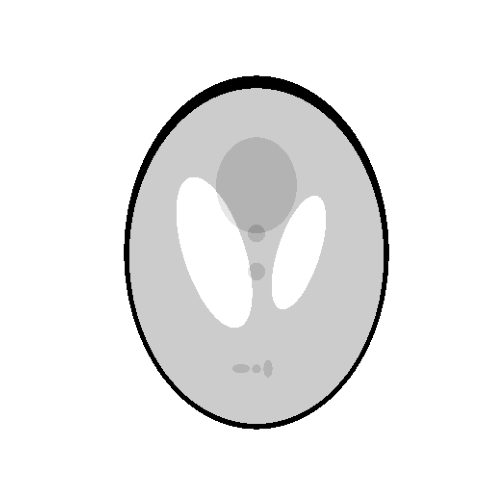
\includegraphics[width=0.18\textwidth]{phantom.png}}
    \subbottom[Original sinogram            \label{fig:ps:phantom_sinogram}]{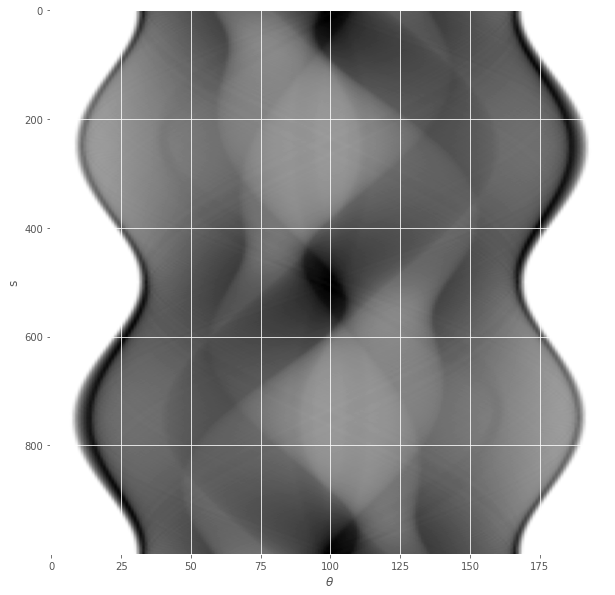
\includegraphics[width=0.18\textwidth]{phantom_sinogram.png}}
    \subbottom[Noisy sinogram               \label{fig:phantom_sinogram_noisy}]{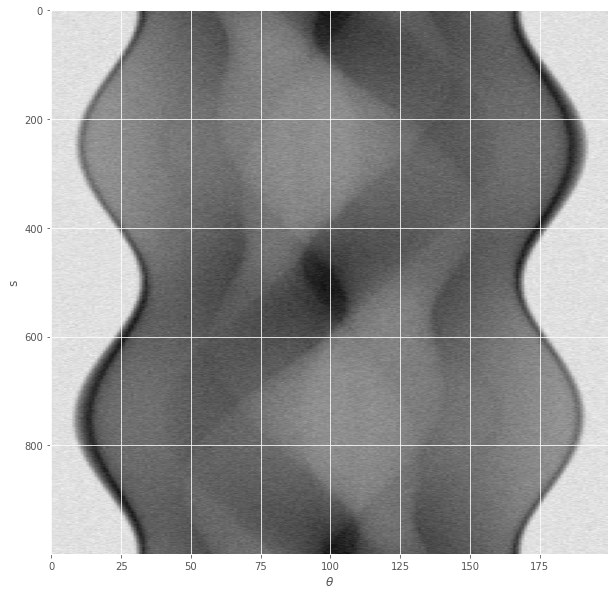
\includegraphics[width=0.18\textwidth]{phantom_sinogram_noisy.png}}
    \subbottom[2nd and 3rd smallest eigenvector of Graph Laplacian      \label{fig:phantom_second_third_evec}]{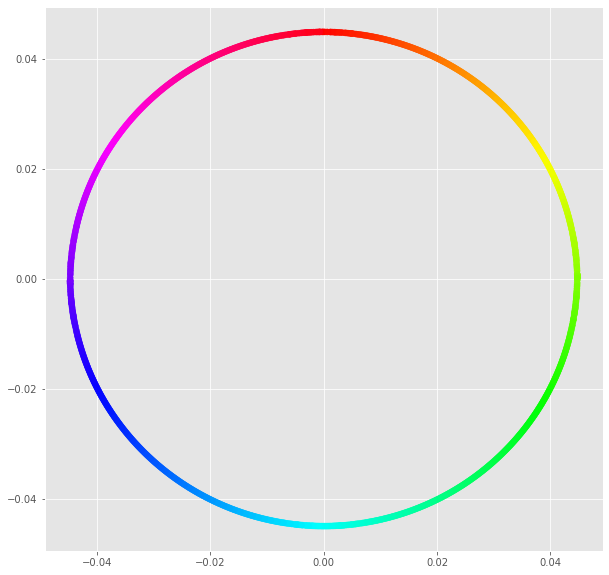
\includegraphics[width=0.18\textwidth]{phantom_second_third_evec.png}}
    \subbottom[2nd and 3rd smallest eigenvector of noisy Graph Laplacian\label{fig:phantom_second_third_evec_noisy}]{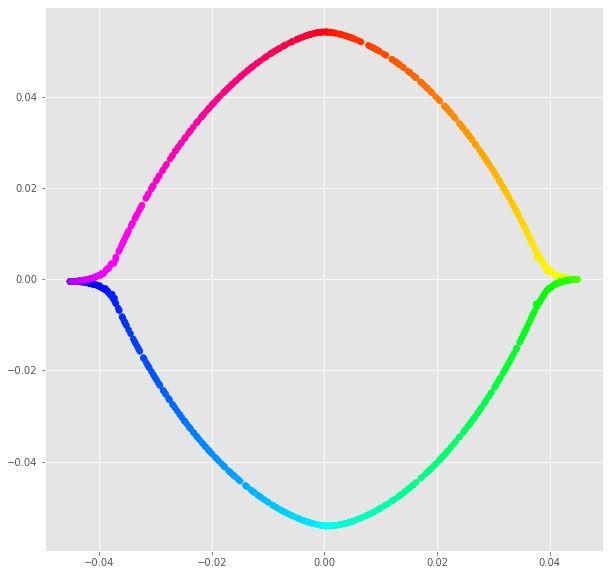
\includegraphics[width=0.18\textwidth]{phantom_second_third_evec_noisy.png}}
    \caption{Shepp-Logan phantom manifold}
\end{figure}

In Figure~\ref{fig:phantom_second_third_evec} the manifold calculated from the original Graph Laplacian
can be seen and it is a perfect circle. Next to it, in Figure~\ref{fig:phantom_second_third_evec_noisy}
the noisy version with $\sigma=2$ is plotted and the manifold is circle like but not at all like from the original one.

The more noise we add, the less the manifold looks like a circle. In Figure~\ref{fig:phantom_second_third_evec_noisy_high}
the manifold for $\sigma=100$ is plotted.

\begin{figure}[H]
    \centering
    \subtop[Highly noisy sinogram               \label{fig:phantom_sinogram_noisy_high}]{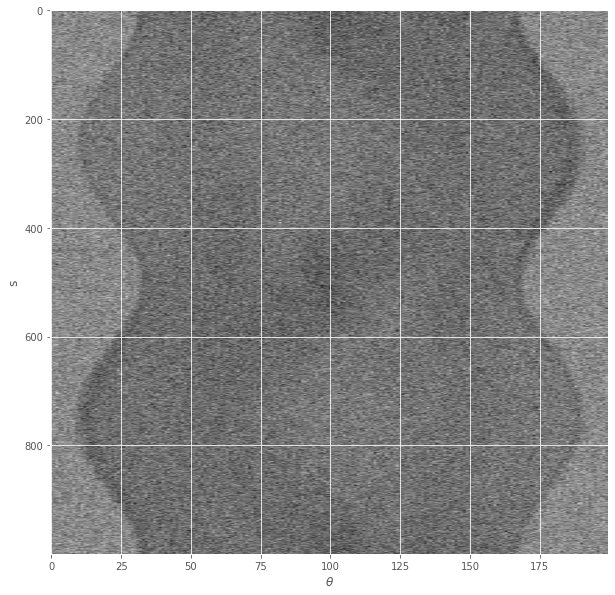
\includegraphics[width=0.4\textwidth]{phantom_sinogram_noisy_high.png}}
    \subtop[2nd and 3rd smallest eigenvector of Graph Laplacian      \label{fig:phantom_second_third_evec_noisy_high}]{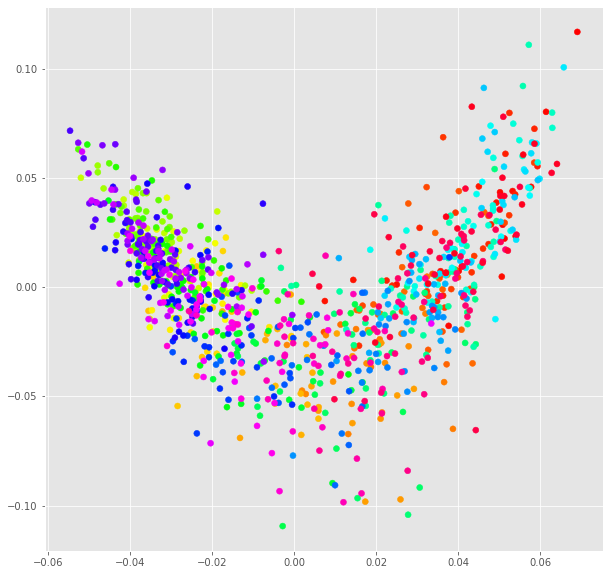
\includegraphics[width=0.4\textwidth]{phantom_second_third_evec_noisy_high.png}}
    \caption{Shepp-Logan phantom manifold for high noise level}
\end{figure}

In all the plots, knn-graph have been constructed with $k=10$. The showed example can be extended to 3D, where the underlying manifold corresponds to the sphere.
Again, the circle and sphere can be computed and for the none-noisy, the underlying manifold can be seen as known.


\section{Thesis problem}
During the Master Thesis, the reconstruction problem with unknown angles is considered. 
Moreover, the observed samples are considered to be noisy. 
The resulting proposed algorithm should work in the 2D and 3D scenario (classical tomography and cryo-Em).

The main idea is to exploit the fact, that the underlying manifold is known (circle in 2D and sphere in 3D). 
From our noisy observations, a manifold can be computed and compare it with the original manifold.
The comparison between the manifolds enables the possibility of a loss function and learning in general.

It is expected, that the folded spectrum \cite{foldedSpectrumMethod} introduced in section~\ref{sec:FoldedSpectrumMethod}
can be used to estimate the eigenvalues of the Graph Laplacian.
Further, as already mentioned in section~\ref{sec:wasserstein-metric}, the wasserstein metric is a good choice
as a loss function when it comes to dealing with data from a manifold distribution \cite{wassersteinGAN}, as in our case. 

The problem can be seen as Graph Denoising as observations are noisy and therefore, the proposed algorithm 
will denoise the graph based on the manifold assumption. 


\paragraph{Evaluation:}
During evaluation, 2D and 3D scenario will be considered. A first evaluation will be done on artificial constructed
toy-dataset. If time allows, real dataset from classical tomography and/or cryo-EM\footnote{https://www.ebi.ac.uk/emdb/} can be evaluated as well.
During evaluation, two baselines are considered which already solved the problem. The first one is a multi-frequency diffusion 
map approach\cite{multiDiffusionMaps, cryoEmMutliDM}, which aims to denoise cryo-EM images. 
Secondly, \cite{LaplaceRandomProjections} a Graph Laplacian approach solving classical tomography with random projection angles will be compare against.
The evaluation process is a first broad idea. Any adjustments in baseline papers or dataset are possible during 
the Master Thesis. The baseline papers are further addressed in the related work chapter~\ref{sec:relatedWork}
and detailed work packages are defined in chapter~\ref{sec:projectPlan}

%\chapter{Related Work}
\label{sec:relatedWork}

In the following section, related work will be introduced.


\section{Graph Deep Learning}
Graph deep learning is a fast evolving field in research. With Graph Neural Networks (GNN)

\cite{GNN}
\cite{GAT}

\subsection{Graph feature extraction with GCN}

\subsection{Graph Convolutional Network}
Graph Convolutional Networks (GCN) \cite{GCN} can be used for many tasks in the field 
of Graph Learning, such as node classification or link prediction. 
Basically, with GCN, a new feature representation is iteratively learned for the node features.

The basic concept is as follows:
For a given graph $G = \langle V,E \rangle$, with node features $X^{N x D}$ and adjacency Matrix $A$
where $N$ denotes the number of nodes and $D$ the number of node input attributes,

a novel node representation $Z^{N x F}$ will be learned, where $F$ is the number of output features.

$Z$ will be learned within a neural network, and every layer can be written by the following, non-linear function:

\begin{equation}
    \begin{aligned}
        H^{l + 1} &= f( H^l, A), \\
        \text{with } H^0 &= X , \\
        H^L &= Z, 
    \end{aligned}
\end{equation}

where $L$ is the number of layers in the neural network.
The model only differ in the choice of $f(\cdot,\cdot)$.

We are ready to define our first GCN. To keep it simple, $f(\cdot,\cdot)$ will be defined as the following:
\begin{equation}
    f( H^l, A) = \sigma (A H^l W^l)
\end{equation} 

Where $\sigma ( \cdot )$ is a non-linear activation function, such as ReLU and $W^l$ is
a weight Matrix of the layer $l$ of the neural network. As \citet{GCN} could show during experiments,
this choice of $f(\cdot,\cdot)$ is already very powerful and leads to state-of-the-art results.

\subsubsection{Renormalization trick}

With this model, we do have two problems and need to refine it further.
First of all, with the multiplication of $A$, we average over the neighbour nodes but
will ignore the node itself. Therefore, self-loops will be added to $A$.
The second problem is, that A is not normalized and if therefore, when multiplying with $A$,
the features of the nodes will change it scale. Therefore, we need to normalize $A$
such that all rows sum to one. This can be done with a simple multiplication with the D.

These two steps are called the Renormalization trick\cite{GCN}.
First of all, we can simple add the self-loops by adding the Identity Matrix to $A$, 
$\hat{A} = A + I$ and $\hat{D}$ is the degree Matrix of $\hat{A}$.
Now, we can achieve a symmetric normalization by multiplying $D^{-\frac{1}{2}} A D^{-\frac{1}{2}}$.

And finally, we can put all things together, and replace $A$ in the original equation:
\begin{equation}
    f( H^l, A) = \sigma (\hat{D}^{-\frac{1}{2}} \hat{A} \hat{D}^{-\frac{1}{2}} H^l W^l)
\end{equation} 


\subsubsection{Simple Graph Convolutional Network}
\textbf{Basically Power method with normalization}

Simple Graph Convolutional Network (SGC) \cite{simpleGCN} proposed a simplified version of GCN.
They could verify their hypothesis, that GCN is dominated by the local averaging step and the non-linear 
activation function between layers do not contribute to much to the success of GCN.

This makes the calculation simpler. We denote $S = \hat{D}^{-\frac{1}{2}} \hat{A} \hat{D}^{-\frac{1}{2}} $
and can use the fact that in every layer of the neural network, the same computation will take place.

\begin{equation}
    \begin{aligned}
        Z = S \dots S X W^1 W^2 \dots W^L \\
        Z = S^L X W^1 W^2 \dots W^L \\
        Z = S^L X W    
    \end{aligned}
\end{equation}

where $W$ is the matrix of all vector weights.



\subsubsection{Link to Graph Laplacian:}

In the section, we will have a look at the connection between SGC and Graph Laplacian.

We can define $x \in R^n$ as our signals and define the Fourier transform as $\hat{x} = U^T x$
and the inverse as $x = U\hat{x}$. 
With the transform, we can easily switch between spatial and Fourier(spectral) domain.

Further, we can define the graph convolution operation between signal $x$ and filter $g$.

\begin{equation}
    g \star x = U((U^T g) (U^T x)) = U \hat{G} U^T x,
\end{equation}

where $\hat{G}$ is a diagonal matrix where the elements are the 
spectral filter coefficients (eigenvalues?)

The graph convolution can be approximated by the $k$-th order polynomials of Laplacians:

\begin{equation}
    \approx \sum_{i=0}^{k} \Delta^i x = U \left ( \sum_{i=0}^{k}  \Theta_i \Lambda^i \right ) U^T x,
\end{equation}

where $\Delta = D - A$ and $\Theta_i$ are 
filter coefficients which correspond to polynomials of the Laplacian eigenvalues,
 $\hat{G} = \sum_i \Theta_i \Lambda^i$


 In the original \cite{GCN} paper, the approximation is done with $k = 1$ 
 \begin{equation}
     g \star x = \Theta (I + D^{-\frac{1}{2}} A D^{-\frac{1}{2}} )x,
 \end{equation}

, where \citet{GCN} further applies the renormalization trick, ending up replacing
$I + D^{-\frac{1}{2}} A D^{-\frac{1}{2}}$ with $\hat{D}^{-\frac{1}{2}} \hat{A} \hat{D}^{-\frac{1}{2}}$.

$I + D^{-\frac{1}{2}} A D^{-\frac{1}{2}}$ is also called first-order Chebyshev filter.

%\footnote{https://towardsdatascience.com/spectral-graph-convolution-explained-and-implemented-step-by-step-2e495b57f801}

%not read currently:
%\footnote{https://towardsdatascience.com/tutorial-on-graph-neural-networks-for-computer-vision-and-beyond-part-2-be6d71d70f49}




\cite{GCN}
\cite{simpleGCN}
\cite{dynamicGCN}



\section{Manifold Learning}
\cite{isomap}
\cite{LLE}
\cite{LaplacianEigenmaps}

\section{Random Walk approaches}

\cite{diffusionMaps}
\cite{vectorDiffusionMaps}
\cite{multiDiffusionMaps}


\section{Denoising}

\subsection{Image Denoising}

\subsubsection{Non local means}
Non local means is a state-of-the-art image denoising method \cite{noneLocalMean}.
In the name of the method are two important concepts, namely the \textit{mean}
and \textit{non local}.

For a given noisy image $v$, the denoised image is defined as:
\begin{equation}
    NL[v](i) = \sum{w(i,j) \; v(j)}
\end{equation}

where $w(i,j)$ is the weight between pixel $i$ and $j$ and fulfils two conditions:
\begin{itemize}
    \item $0 \le w(i,j) \le 1$
    \item $\sum_j{w(i,j) = 1}$
\end{itemize}

The weight can be seen as a similarity measure of the two pixels.
Moreover, these similarities are calculated over square neighbourhoods of the two pixels,
where the l2 norm of the neighbourhood is used.
Similar pixel neighbourhoods have a large weight and different neighbourhoods have a small weight.

More general, the denoised image pixel $i$ is computed as an weighted average of all pixels in the 
image, therefore, in a non local way.
Image Denoising
Graph Denoising

\subsection{Graph Denoising}

\cite{noneLocalMean}
\cite{learningToDrop}


\subsection{cryo-EM calcuation}

\section{Graph Laplacian Tomography From Unknown Random Projections}

\citet{LaplaceRandomProjections} introduces a Laplacian-based algorithm, with which 
reconstruction of a planar object from projects at random unknown directions is possible.

Overall, in computerized tomography (CT), reconstruction of an object with only samples of its projections
is a standard problem. In \citet{LaplaceRandomProjections} the problem was extended by the fact,
that the projection angle to the object is unknown.

Formally:
Given $N$ projection vectors $( P_{\theta_i}(t_1), P_{\theta_i}(t_2), \dots, P_{\theta_i}(t_N)$ 
at unknown angles $\{\Theta_i\}^N_{i=1}$ which are drawn from the uniform distribution of $[0, 2\pi]$
and $t_1, t_2, \dots, t_n$ are fixed n points (all equally spaced due to uniform distribution) 
find the underlying density function $\rho (x,y)$ of the object.

\subsection{Radon transform}

The radon transform $P_{\Theta}(t)$ is the line integral of $\rho$
along parallel lines $L$ at angle $\Theta$ and distance $t$ from the orign.

\begin{equation}
    \begin{aligned}
        P_{\Theta}(t) &= \int_L \rho (x,y) ds \\
                      &=  \int_{-\infty}^{\infty} \rho (x,y) \; \delta(x \cos \Theta + y \sin \Theta - t) dx \; dy
    \end{aligned}
\end{equation}

An algorithm for estimating angles from given projections have been introduced by \cite{formerUnkownRandomProjections}.
The introduced algorithm consists of three steps:
\begin{enumerate}
    \item Angle estimation
    \item Angle Ordering
    \item Joint maximum likelihood refinement of angles and shifts
\end{enumerate}

Step 2 was implemented by some nearest neighbour algorithm. In the work of 
\cite{LaplaceRandomProjections}, they introduced a new way of ordering the angles,
using Graph Laplacian.


\subsection{Laplace-Beltrami operator}
\cite{LaplaceRandomProjections} could show, that the graph Laplacian
 approximates the Laplace-Beltrami operator, if data points are uniformly distributed 
 over the manifold.

 Further, they showed that in the case of non-uniformly distributed data points, the Laplacian
 approximated the backward Fokker-Planck operator (which is a generalization of the Laplace-Beltrami operator).
 With that, at least the ordering of the angles can be estimated.

 Finally, with a small normalization of the Laplacian, the Laplace-Beltrami operator can also be 
 approximated in the non-uniform distributed case.

\subsection{Algorithm}

For a given set of projections vector $x_i = ( P_{\Theta_i}(t_1), \dots, P_{\Theta_i}(t_n))$ for $i = 1,2, \dots, mN$

The algorithm proposed in \cite{LaplaceRandomProjections} consists of five steps:

\begin{enumerate}
    \item Double the number of projections to 2mN (due to the fact that projections are symmetric)
    \item Construct the co-called density invariant Graph Laplacian $\tilde{L}$
    \item Compute $\theta_1(i)$ and $\theta_2(i)$ the first two nontrivial eigenvector of $\tilde{L}$
    \item Sort $x_i$ according to $\phi_i = \tan^{-1}(\theta_1(i) \; / \;\theta_2(i))$
    \item Reconstruct image using the sorted projections and estimated angles.
\end{enumerate}

Where $\tilde{L}$ can be constructed by the following way:

\begin{equation}
    \begin{aligned}
        W_{ij} = k \left ( \frac{\left \| x_i - x_j \right \|^2}{2 \epsilon}  \right ), \\
        i, j = 1, \dots, N
    \end{aligned}
\end{equation}

where $||\cdot ||$ is the euclidean-norm, $k$ a semi-positive kernel 
and  $\epsilon > 0$ the bandwidth of the kernel. As mentioned in \cite{LaplaceRandomProjections},
the kernel $k(x) = \exp (-x)$ is a popular choice.

With the newly computed weight Matrix $W$ and the degree Matrix $D$ corresponding to $W$, we can finally 
define $\tilde{L}$.

\begin{equation}
    \begin{aligned}
        \tilde{W} &= D^{-1} W D^{-1} \\
        \tilde{D} &= \text{Degree matrix corresponding to } \tilde{W} \\
        \tilde{L} &= \tilde{D}^{-1} \tilde{W} - I \\
    \end{aligned}
\end{equation}


%\chapter{Evaluation}
\label{sec:evaluation}


Create artificial data to test algortihm
and add hand crafted noise.

Use CT tomography for simple 2D tomography case.
Shepp-Logan phantom.

Long view, application to cryoEM, 
but probably not possible during MS Thesis.

Baseline Papers

Multifrequency Vector diffusion maps \cite{multiDiffusionMaps}

and \cite{LaplaceRandomProjections}
%\chapter{Master Thesis project}
\label{sec:projectPlan}
In the last chapter of the Thesis Preparation report, the project plan will be introduced as well as a broad overview of different 
work packages. Further, the project timeline can be seen as a Gantt chart.
Probably, there are some parts which will not work out as expected and 
adjustments are needed throughout the Thesis, the project plan can be seen as a rough guideline.

\section{Problem conclusion:}
Conlusion from red boxes


\section{Work packages}

\paragraph{Implement algorithm for 2D case:}
The first step will be, to familiarize with the problem and implement
the algorithm for 2D. 

\paragraph{Evaluate 2D case on toy dataset and implement baselines:}
As a second step, the implemented 2D algorithm will be tested on a toy dataset,
where noise is added to the images by hand. As the aim is to work with highly noisy images,
the noise level can be selected and increased when working with toy datasets. 
The evaluation in 2D is crucial and needs to in a satisfying matter. 
It does not make sense to continue with 3D implement, when the simply 2D case is not handled well enough.
Therefore, if the evaluation results are not satisfying, the algorithm needs to be iteratively adjusted, 
such that the evaluation will be in a good enough quality.


\paragraph{Implement algorithm for 3D case:}
After successfully evaluating the algorithm in 2D, the aim is to extend the algorithm to work in 3D as well.

\paragraph{Evaluate 3D case on toy dataset and adjust baselines:}
Again, the implementation will be evaluated on a toy dataset, where noise can be adjusted by hand.


\paragraph{Nice to have: Evaluate of real dataset}
If time allows and the 2D and 3D implementation are evaluated successfully on toy datasets, 
real data can be used for further evaluation. This step will only be done, if time allows.


\paragraph{Evaluate related work:}
As cryo-EM reconstruction is a hot research topic, related work can not only
be considered during the start of the Thesis and needs to be evaluated throughout the Thesis.

\paragraph{Writing Thesis:}
Document implementation and evaluation result.

\begin{landscape}

    \section{Gantt chart}

    \newganttchartelement{bluebar}{
    bluebar/.style={
        inner sep=0pt,
        draw=purple!44!black,
        very thick,
        top color=white,
        bottom color=blue!80
    },
    bluebar label font=\slshape,
    bluebar left shift=.1,
    bluebar right shift=-.1
}

\newganttchartelement{greenbar}{
    greenbar/.style={
        inner sep=0pt,
        draw=green!50!black,
        very thick,
        top color=white,
        bottom color=green!80
    },
    greenbar label font=\slshape,
    greenbar left shift=.1,
    greenbar right shift=-.1
}

\ganttset{%
calendar week text={W\currentweek}%
}

    
    \begin{adjustwidth}{-70pt}{}
        \begin{ganttchart}[expand chart=1.8\textwidth,
            hgrid style/.style={black, dashed},
            vgrid={*{6}{draw=none},dotted},
            x unit=3pt,
            y unit chart=20pt,
            time slot format=isodate,
            group label font=\bfseries \Large,
            ]{2021-12-01}{2022-05-29}
            \gantttitlecalendar{year, month=name, week}{1}\\
        
            \ganttgroup[ group/.append ]{2D classical tomography}{2021-12-01}{2022-02-13}\\ 
                \ganttbluebar[name=Implementation 2D]{Implementation in 2D}{2021-12-01}{2022-01-09}\\ 
                \ganttbluebar[name=Implement Baselines]{Implement Baselines for 2D Evaluation}{2022-01-10}{2022-01-23}\\ 
                \ganttbluebar[name=Evaluation 2D]{Evaluation 2D on toy dataset}{2022-01-24}{2022-02-13}\\ 
                \ganttbluebar[name=Related Work]{Related Work}{2022-01-01}{2022-01-10}\\ 
                \ganttgreenbar[name=Honeymoon]{Honeymoon}{2021-12-20}{2022-01-10}
                
            \ganttnewline[thick, black]

            \ganttgroup[ group/.append]{3D cyro-EM}{2022-02-13}{2022-04-10}\\ 
                \ganttbluebar[name=Implementation 3D]{Implementation in 3D}{2022-02-14}{2022-03-06}\\ 
                \ganttbluebar[name=Extend Baselines 3D]{Extend Baselines for 3D Evaluation}{2022-03-07}{2022-03-20}\\ 
                \ganttbluebar[name=Evaluation 3D]{Evaluation 3D on toy dataset}{2022-03-21}{2022-04-10}
            
                \ganttnewline[thick, black]
        
            \ganttgroup[ group/.append ]{Finalization}{2022-04-11}{2022-05-29}\\ 
                \ganttbluebar[name=Final Evaluation Result]{Final Evaluation Results}{2022-04-11}{2022-04-24}\\ 
                \ganttbluebar[name=Thesis]{Writing Thesis}{2022-04-25}{2022-05-29}\\
                \ganttgreenbar[name=Fatherhood]{Birth of first child}{2022-04-20}{2022-04-27}
        
            %Implementing links
            \ganttlink[link bulge=2, link mid=0.5]{Implementation 2D}{Implement Baselines}
            \ganttlink[link bulge=2, link mid=0.5]{Implement Baselines}{Evaluation 2D}
            
            \ganttlink[link bulge=2, link mid=0.5]{Evaluation 2D}{Implementation 3D}
        
            \ganttlink[link bulge=2, link mid=0.5]{Implementation 3D}{Extend Baselines 3D}
            \ganttlink[link bulge=2, link mid=0.5]{Extend Baselines 3D}{Evaluation 3D}
            
            %\ganttlink[link bulge=0.5, link mid=0.01]{Implementation 2D}{Clean-Up}
            %\ganttlink[link bulge=2, link mid=0.3]{Implementation 3D}{Clean-Up}
        
        
            \ganttlink[link bulge=2, link mid=0.5]{Evaluation 2D}{Final Evaluation Result}
            \ganttlink[link bulge=2, link mid=0.5]{Evaluation 3D}{Final Evaluation Result}
            \ganttlink[link bulge=2, link mid=0.5]{Final Evaluation Result}{Thesis}
        
        \end{ganttchart}
        \end{adjustwidth}

\end{landscape}

%% ----------------------------------------------------------------
%\thesisappendix
\thesisbib
\begin{appendices}
	% !TEX root = ../Thesis.tex
\chapter{Mathematical tools}
\section{Power Iterations}
\label{sec:powerIterations}

Power iteration (also called power method) is a iteratively method, 
which approximates the biggest eigenvalue of a diagonalizable matrix $A$.

The algorithm starts with a random vector $b_0$ or an approximation of the dominant eigenvector.

\begin{equation}
    \label{eq:powerIterations}
    b_{k+1} = \frac{Ab_k}{||Ab_k||}
\end{equation}

\textbf{TODO:convergence if there is only one largest eigenvalue and if b0 is not orthogonal to the eigenvector associated with the largest eigenvalue.}

The algorithm not necessarily converges. The algorithm will converge, if $A$ has an eigenvalue strictly grater than its other eigenvalues
and the initial vector $b_0$ has a component in direction of an eigenvector, associated with the dominant eigenvector.

\section{Folded spectrum Method}

\textbf{TODO: I don't know what is the Hamiltonian matrix, so either you define it or don't talk about it. 
You can also introduce the folded spectrum just as a way to recover the eigenvector associated with a known eigenvalue. Epsilon often refers to a very small scalar.}


\label{sec:FoldedSpectrumMethod}
Calculation of eigenvalues and eigenvectors of a given Hamiltonian matrix $H$ 
is a fundamental mathematical problem. Often, we are interested in just the smallest 
values, which can be efficiently computed. But if we are interested in selected values,
this can be hard. $H$ is needed to be diagonalized (bring matrix $H$ into diagonal form) 
which is computationally expensive and for big matrices impossible.

Currently, the best way to solve such problems is the Folded spectrum (FS)\cite{foldedSpectrumMethod} method,
which iteratively solves the problem. During calculation, the eigenvalue spectrum will be folded around a reference 
value $\epsilon$.

\begin{equation}
    \label{eq:foldedSpectrumMethod}
    v^{t+1} = v^t - \alpha (H - \epsilon I )^2 v^t ,
\end{equation}

with $0 < \alpha < 1$. When $t \rightarrow \infty$, then $v^{\infty}$ will be the 
eigenvector with respect to the reference value $\epsilon$.


\section{Wasserstein metric}
\label{sec:wasserstein-metric}
\textbf{TODO: the difference between Wasserstein and KL divergence for instance is that it is defined (the value is finite) even if the two distributions have not the same support. }


The Wasserstein metric is a distance measure between two probability distributions and it is used in ML as a loss function\cite{learningWithWasserstein}. 
Intuitively, it can can be understood as the minimum cost to transfer the mass of one distribution to the other.
Therefore, it is also known as the \textit{earth mover's distance}.

As \citet{wassersteinGAN} could show, ordinary distance measures like \textit{Total Variation}, \textit{Kullback-Leibler divergence}
and \textit{Jensen-Shannon divergence} are not sensible when learning with distributions supported by manifolds
On the contrary, Wasserstein metric does a good job as loss function in such scenarios.


\section{Fourier Transform}
\textit{Fourier Analysis} is the overall field of study, which deals with representing (or approximating) functions as 
sums of trigonometric functions. When the function is defined in such a way, we are talking from the \textit{Fourier Domain}.

\textit{Fourier transform} (FT) is the way of transforming signals to the Fourier Domain, which is popular in ML.
Basically, with the Fourier transform, a signal can be decomposed to a \textit{Fourier series}, which consists of many weighted sinusoids. 

\paragraph{Fourier-slice theorem}
The Fourier-slice theorem \cite{fourierSliceTheorem} in 3D is defined as follows:

\begin{equation}
    \label{eq:Fourrier-slice}
    F_2 P_2 = S_2 F_3,
\end{equation}

where $F2$ and $F3$ are FTs in 2D and 3D respectively, P2 is a projection operator ($P_2 : 3D \rightarrow 2D$) and $S2$ is the restriction operator.

As pointed out by \cite{cryoEmMath},
the Fourier-slice theorem is the foundation of the reconstruction problem in computerized tomography (CT), which will be explained in section~\ref{sec:reconstructionProblemCT}.
It states, that the 2D FT of the tomographic projection is the same as the 3D FT restricted to a 2D plane through the origin.
Basically, for the CT reconstruction problem, acquiring samples from known viewing directions is the same 
as sampling the 3D Fourier-space. This concept is exploited by the filter BackProjection algorithms, see section~\ref{sec:filterBackProjection}.

\section{Radon Transform}
The radon transform\cite{radonTransform} is the main mathematically concept of tomographic reconstruction.

It is an integral transformation of a function $f(x,y)$, which is defined on the plane. In tomographic reconstruction
the function $f$ will be the observed tomographic image.
The radon transform then transforms $f$ to a function $Rf$, which corresponds to the line integral of the line defined by 
the two parameters $\theta$ and $s$, where $\theta$ is a angle and $s$ the distance to the origin.

In Figure~\ref{fig:phantom_theta45} and Figure~\ref{fig:phantom_theta45_s14} on can see two plots of different
values for $\theta$ and $s$, where $f(x,y)$ is the Shepp-Logan phantom. The complete $R(\theta=45, s=0)x$, 
which is also called \textit{sinogram}, can be see in Figure~\ref{fig:phantom_sinogram}

\begin{figure}[H]
    \centering
    \subbottom[Radon Transform  $R(\theta=45, s=0)x$\label{fig:phantom_theta45}]{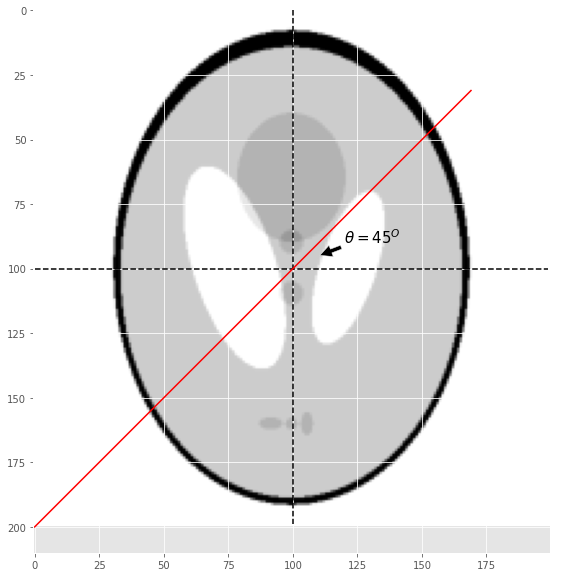
\includegraphics[width=0.3\textwidth]{phantom_theta45.png}}
    \subbottom[Radon Transform  $R(\theta=45, s=14.14)x$\label{fig:phantom_theta45_s14}]{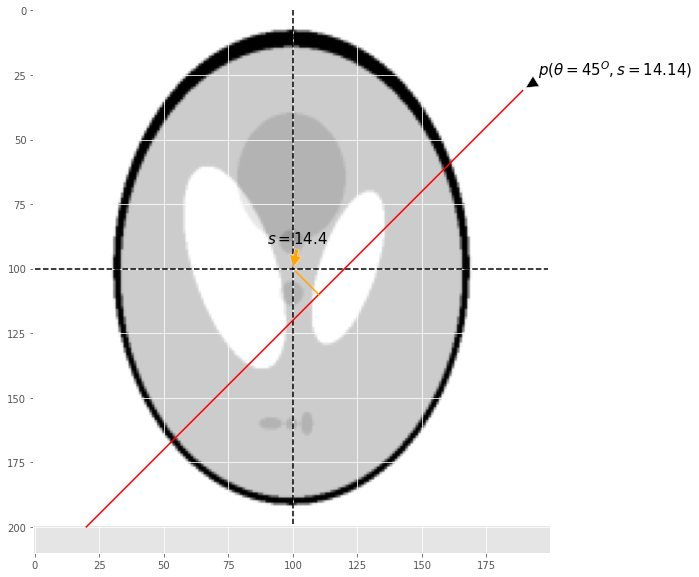
\includegraphics[width=0.3\textwidth]{phantom_theta45_s14.png}}
    \subbottom[Shepp–Logan phantom sinogram of $R(\theta=45, s=0)x$\label{fig:phantom_sinogram}]{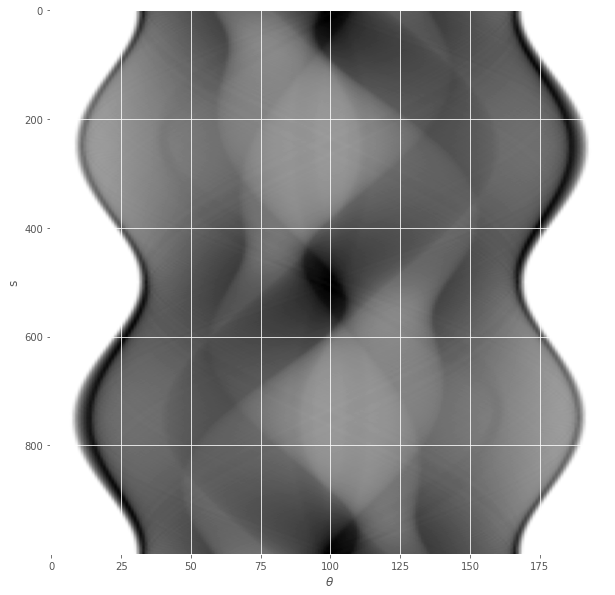
\includegraphics[width=0.3\textwidth]{phantom_sinogram.png}}
    \caption{Examples, where the original object $x$ is the Shepp-Logan phantom.}
\end{figure} 
\end{appendices}
%% ----------------------------------------------------------------
\thesisback
%\iflanguage{english}
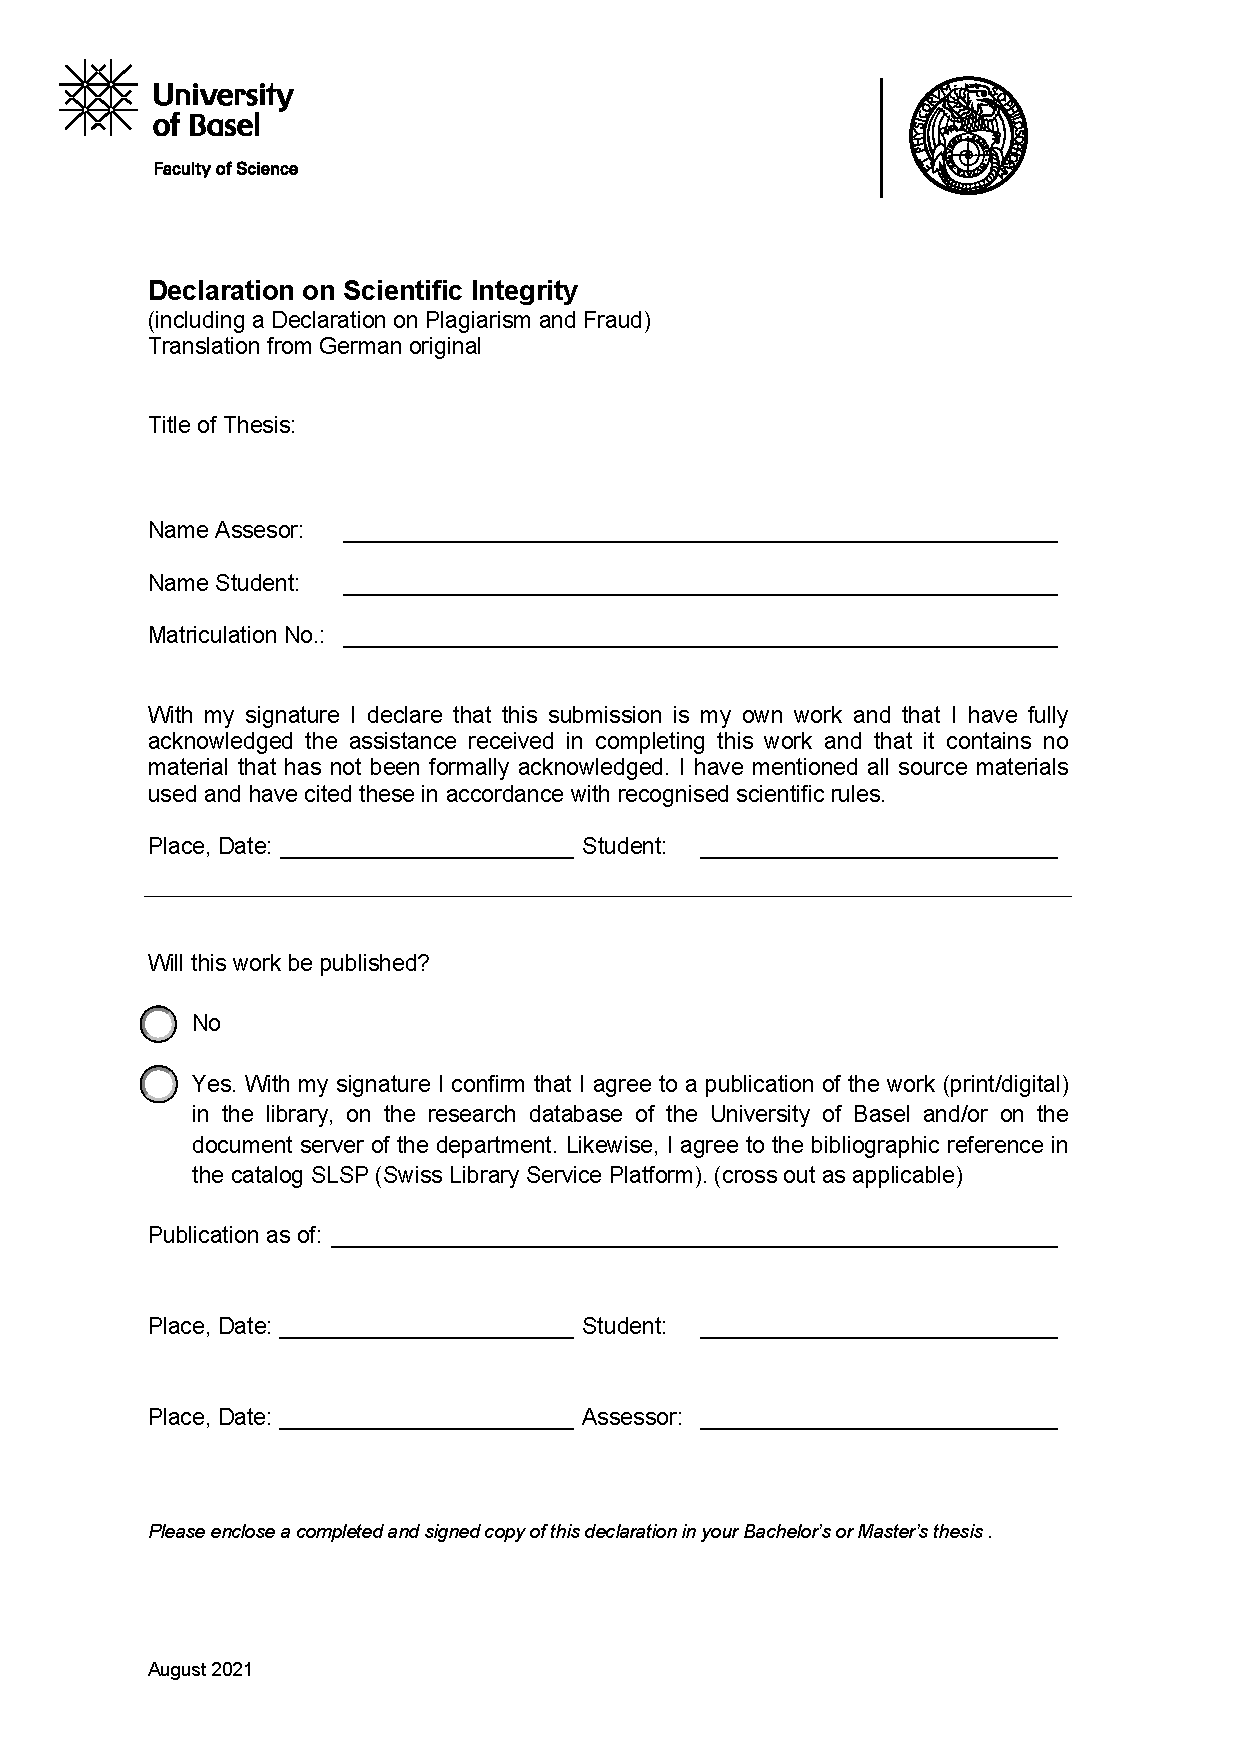
\includepdf{./Back/wissensch_Redlichkeit_E_Aug_21.pdf}
%  {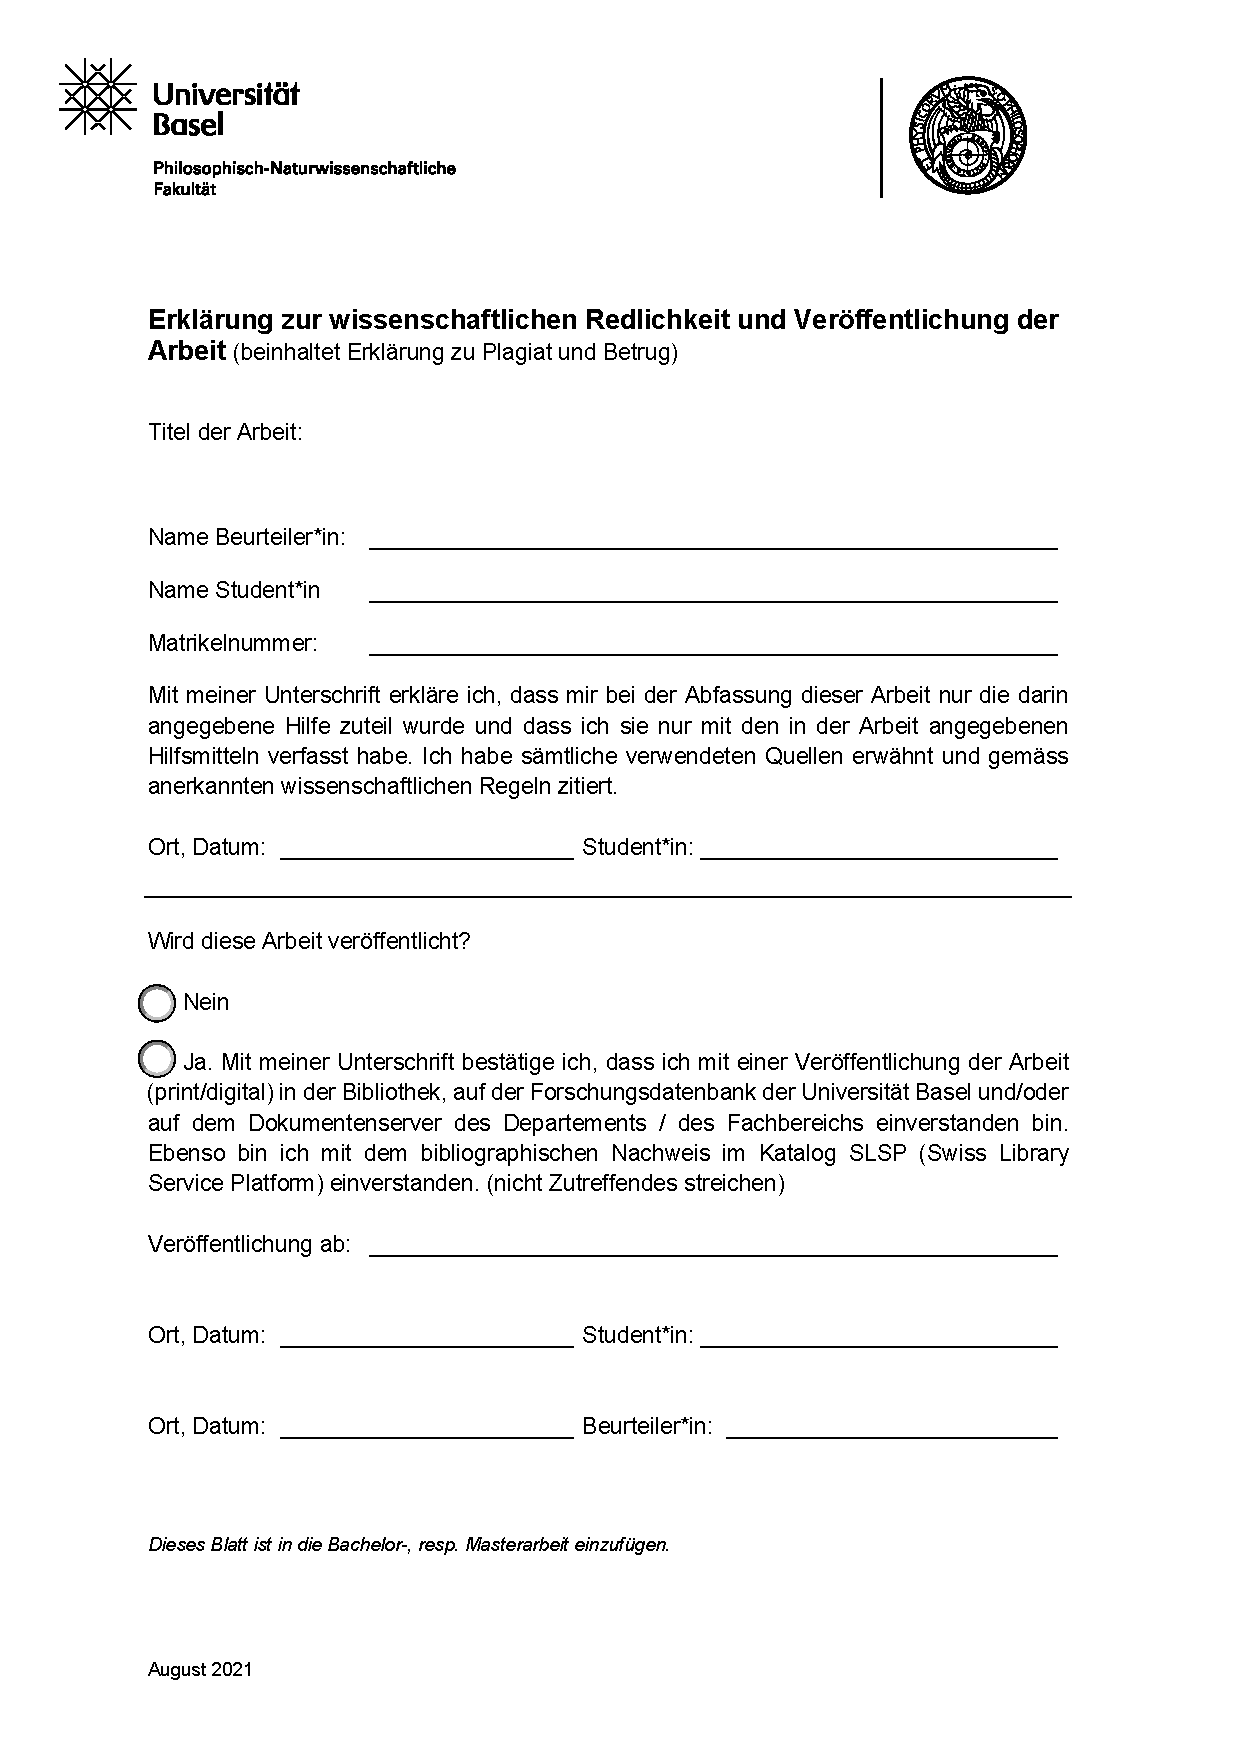
\includepdf{./Back/wissensch_Redlichkeit_D_Aug_21.pdf}}
%% ----------------------------------------------------------------
\end{document}
%% ----------------------------------------------------------------
